\documentclass[11pt,letterpaper, notitlepage]{article}
\usepackage{epsf,graphicx,psfrag}
\usepackage{natbib}
\usepackage{setspace}
\usepackage{fullpage}
\usepackage[reqno]{amsmath}
\usepackage{endnotes}
\usepackage{natbib}
\usepackage{amsfonts}
\usepackage{amssymb,enumerate}
\usepackage{dcolumn}
\usepackage{verbatim}
%\usepackage{hypertex}
\usepackage[pdftex, bookmarks, colorlinks=true, plainpages = false, citecolor = blue, urlcolor = blue, filecolor = blue, breaklinks]{hyperref}
\usepackage{amssymb}
\usepackage{amsmath}
\usepackage[hmargin=3.0cm,vmargin=3.0cm]{geometry}
%\usepackage{geometry}
\usepackage{nicefrac}
\usepackage{pdfsync}
\usepackage{url}
\usepackage{pst-all}
\usepackage{pdflscape}
\usepackage{rotating}
\usepackage[T1]{fontenc}
\usepackage[sc]{mathpazo}
\usepackage{graphicx,verbatim,scalefnt}

\newtheorem{definition}{Definition}
\newcommand{\ta}{\theta}
\newcommand{\Ta}{\Theta}
\newcommand{\ga}{\gamma}
\newcommand{\un}{\underline}
\newcommand{\ov}{\overline}
\newcommand{\de}{\delta}
\newcommand{\ve}{\varepsilon}
\linespread{1.05} % Palatino needs more leading (space between lines)
\title{Unrecognized States: A Theory of Self-Determination and Foreign Influence}

\author{Kristy Buzard\\
Syracuse University\\
\\
Benjamin A.T. Graham \\
University of Southern California\\
\\
Ben Horne\\ 
University of California, San Diego}

\date{\today}
\begin{document}
\begin{titlepage}
\maketitle
\thispagestyle{empty}
\center{This article is a working paper and is subject to future revision during the peer-review process. The authors welcome any comments, and may be reached by e-mail at benjamin.a.graham@usc.edu.}

\begin{abstract}
\noindent Unrecognized states are characterized by stagnant or crumbling economies and political instability, often serve as havens for illicit trade, and challenge the territorial sovereignty of recognized states. Their persistence is both intellectually puzzling and normatively problematic, but unrecognized statehood can be a remarkably stable outcome, persisting for decades. Our dynamic four-player model reveals that unrecognized statehood emerges as an equilibrium outcome when a patron state is willing and able to persistently invest resources to sustain it. %Counterintuitively, patrons will make these investments even when unrecognized statehood is not their most preferred outcome. 
We assess options available to actors in the international community who seek to impose their preferred outcomes in these disputes and find that, although sanctions are the most frequently employed, they can often lead to renewed conflict instead of the intended resolution.
\end{abstract}

\end{titlepage}
\setcounter{page}{1}

\doublespacing
\section{Introduction}
South Ossetia is an archetypical unrecognized state -- characteristic of those regions of the world in which non-state actors control territory and govern populations. From 1990 to 1992, Ossetian rebels fought a successful secessionist civil war against the Georgian government that ended with a ceasefire and left the rebels in \textit{de facto} control of much of the region of South Ossetia, which sits along Georgia's northern border with Russia. In the 22 years since the ceasefire was signed, South Ossetia has functioned as an unrecognized state, governing its own affairs but unrecognized by foreign nations.\footnote{South Ossetia, along with Abkhazia, was recognized by Russia and Nicaragua in 2008, Venezuela and Nauru in 2009, and Tuvalu in 2011.} The Georgian government maintains its claim to the territory of South Ossetia, while the South Ossetians continue to seek international recognition of their independence. In 2004, the Georgian government began intermittent efforts to close trade with the separatist region, and in 2008, following escalating provocations from the Ossetian side, Georgia attempted to reclaim the territory by military force. Russian troops acting in support of the Ossetians quickly crushed the would-be reconquest, and the status quo was restored.%\footnote{Good sources on the history of the conflict include Lynch 2004, Asmus 2010, and a series of reports by the International Crisis Group.}

The international system is characterized by a norm under which seceding entities are rarely recognized by foreign states unless they are first recognized by the home state.\footnote{This norm is not absolute: in some cases, like the People's Republic of China, the sovereignty of the home state government (over Taiwan) has never been recognized by some states. In other cases, like Kosovo, the commission of mass atrocities by the home state government may supersede its sovereignty.} This norm makes sense in a context where almost all states have reason to fear the emergence of secessionist movements within their own borders, and a state system that places seceding entities at an extreme disadvantage lowers the expected benefits of secession, thereby reducing the incentives for secessionist movements.\footnote{Coggins (2011: 451) notes that, "The more acute the domestic threat, the more the reticence to recognize." For the definitive international legal treatment of recognition, see Crawford (2006).}%The higher the costs of secession, the greater the security of existing states. 
Thus, unrecognized states emerge when seceding entities gain \emph{de facto} territorial control through successful wars of secession, but are not militarily strong enough to force recognition of their independence from the home state from which they have seceded.

Persistent unrecognized statehood is both intellectually puzzling and normatively undesirable. It is an extremely costly outcome for the secessionists, the home states from which they are attempting to secede, and the international community more broadly. Nonetheless, unrecognized statehood has been a recurring phenomenon since WWII, with half a dozen current unrecognized states having existed for more than 20 years.\footnote{Abkhazia, Ngorno-Karabakh, Transnistria, Somaliland, South Ossetia, and the Turkish Republic of Northern Cyprus.} Much of the existing literature treats unrecognized statehood as either a transient phenomenon or simply as a failure to reach recognized statehood. In contrast, we argue that unrecognized statehood is an important outcome in its own right, and one that is potentially extremely stable over time. A major contribution of this paper is the demonstration of unrecognized statehood as a long-run equilibrium outcome of the strategic interaction between not just the secessionists and the home government, but also the international community and states or non-state actors who act as patrons of the secessionists. We show that unrecognized statehood can be a stable outcome despite its persistently high costs to all actors involved.

The costs to the secessionists are arguably the highest. Non-recognition locks unrecognized states out of a states-only club whose members enjoy benefits in terms of both security and economic integration. Unrecognized states do not benefit from the norm of territorial integrity that reduces the cost of territorial defense by increasing the chance that foreign powers will intervene against, or at least sanction, an invader.\footnote{See Zacher (2001) on the norm of territorial integrity.} Non-recognition also prevents entry into multilateral and bilateral trade agreements, dramatically reduces access to foreign aid, and excludes their territory from international legal frameworks, making it harder to secure foreign investment (Milhalkanian 2004; Caspersen 2013: 40-45).\footnote{Transnistria represents a case where the gains from smuggling, particularly for the elite, may have outweighed these other economic costs in the 1990s (King 2001). However, as Moldova deepens ties with the EU, Transnistria's lack of access to EU markets and EU aid becomes a much larger relative cost to bear (Tudoroiu 2011).} %In their most direct form -- loans and foreign aid -- these benefits are referred to as ``rents to sovereignty" (Collier and Hoeffler 2005). 

The home state bears costs of non-settlement as well, although they are not as high as those facing the unrecognized state. Instability in the border region and the diversion of military resources to monitor the \textit{de facto} border are costly, as is maintenance of economic sanctions against the unrecognized state. In Azerbaijan, where an oil boom sent GDP soaring in the mid-2000s, the unresolved secessionist conflict in Nagorno-Karabakh led a massive military buildup to take precedence over other government spending.\footnote{Military spending increased 51\% in 2004-2005, and went up another 82\% in 2006 (International Crisis Group 2007)} Foreign investors are more wary of investing in states that do not effectively control their own territory, and there are diplomatic costs as well. For Georgia, failure to resolve its outstanding secessionist conflicts has hindered progress toward NATO accession.

%Unrecognized statehood is a thorn in the side of the state system. Many unrecognized states are havens for smuggling and trafficking illicit goods, they are prone to violent conflict, and their very existence challenges the norm of territorial sovereignty (King 2001; Stanislawski 2008). Like most unrecognized states, South Ossetia pays high costs for non-recognition. Its political survival is tenuous, its licit economy is in shambles after years of isolation and instability, and yet, if the history of similar entities are any guide, its chances of eventual recognition are slim. Stalemate imposes similar, though less severe, costs on home states (e.g. Georgia) as well.





%\subsection{Non-Recognition and Its Costs}
%Since WWII, the path to recognized statehood has been narrow, and securing territorial control is not sufficient to gain recognition. The international community has been exceedingly clear that a national right of self-determination applies only to cases of decolonization: it does not extend to cases of secession.  In 1970, UN secretary general U Thant said, ``The United Nations has never accepted and does not accept and I do not believe will ever accept the principle of secession of a part of its member states."\footnote{Pegg 1998: 8} In cases where the home state's sovereignty is disputed or where the home state government commits mass atrocity crimes, some states may choose to grant recognition, but there remains a strong norm of home-state veto.That is, secessionist entities are rarely recognized by foreign states unless they are first recognized by the home state from which they are attempting to secede.  This has lead to the existence of an odd group of state-like entities that control territory and govern population but are not recognized as states and cannot participate in the international system. We refer to these entities as unrecognized states, though, variously specified, they are also referred to states-within-states\footnote{Kingston and Spears 2004} \textit{de facto} states,\footnote{Pegg 1998, Lynch 2004} or almost-states.\footnote{Stanislawski 2008}

%Since WWII, the path to recognized statehood has been narrow, and securing territorial control is not sufficient to gain recognition. Seceding entities are rarely recognized by foreign states unless they are first recognized by the home state from which they are attempting to secede.\footnote{This norm is not absolute: in some cases, like the People's Republic of China, the sovereignty of the home state government (over Taiwan) has never been recognized by some states. In other cases, like Kosovo, the commission of mass atrocities by the home state government may supersede its sovereignty.} This norm of home state veto emerges because almost all states have reason to fear the emergence of secessionist movements within their own borders, and a state system that places seceding entities at an extreme disadvantage lowers the expected benefits of secession, thereby making secession less likely.\footnote{Coggins (2011: 451) notes that, "The more acute the domestic threat, the more the reticence to recognize."} The higher the costs of secession, the greater the security of existing states.



%Unrecognized statehood is a particularly compelling outcome from secession in part because while the secessionists have succeeded in securing control of (most of) the territory they aspire to rule they are not recognized by most other states, trapping them in a costly limbo. 

%Unrecognized states are subject to high costs of non-recognition generated by an international system extremely hostile to non-state territorial units. The modern state system is based on institutions designed to facilitate peaceful and economically beneficial relations between like actors, and on the empowerment and legitimation of states through mutual recognition (Spruyt 1996). The norm challenged most directly by unrecognized states is that which, in the post-WWII era, has become most fundamental to it -- the norm of territorial sovereignty. Almost all states have reason to fear the emergence of secessionist movements within their own borders, and a state system that places seceding entities at an extreme disadvantage lowers the expected benefits of secession, and thereby makes secession less likely.\footnote{Coggins (2011: 451) notes that, "The more acute the domestic threat, the more the reticence to recognize."} The higher the costs of secession, the greater the security of existing states.

%The most direct manifestation of this systemic hostility to secession is the norm of states refusing to recognize a seceding entity unless the home state recognizes it first.\footnote{For a thorough international legal discussion of the issue, see Crawford 2006.} This norm is not absolute: in some cases, like the People's Republic of China, the sovereignty of the home state government (over Taiwan) has never been recognized by some states. In other cases, like Kosovo, the commission of mass atrocities by the home state government may supersede its sovereignty. However, the norm is strong and gives recognition by the home state its significance: without recognition by the home state, the post-WWII norm is for other states is to withhold recognition as well.\footnote{Caspersen (2012) traces the history of collective non-recognition, which begins after WWI and solidifies after WWII. In terms of the model presented below, the payoff from territorial control before WWI was equivalent to the payoff from recognized statehood. Players did not need to participate in the game described in the model. We limit our discussion to the post-WWII era, when the norm of home state veto is fully developed.} 

%Abkhazia, Ngorno-Karabakh, Transnistria, Somaliland, South Ossetia, and the Turkish Republic of Northern Cyprus have all controlled territory for over a decade without gaining recognition by more than four other states.

%Non-recogition locks unrecognized states out of a states-only club whose members enjoy benefits in terms of both security and economic integration. For recognized states, the norm of territorial integrity lowers the cost of territorial defense by increasing the chance that foreign powers will intervene against, or at least sanction, an invader.\footnote{See Zacher (2001) on the norm of territorial integrity.} Recognition also allows entry into multilateral and bilateral trade agreements, dramatically bolsters access to foreign aid, and incorporates territory into international legal frameworks that make it easier to secure foreign investment (Milhalkanian (2004); Caspersen 2012: 40-45).\footnote{Transnistria represents a case where the gains from smuggling, particularly for the elite, may have outweighed these other economic costs in the 1990s (King 2001). However, as Moldova deepens ties with the EU, Transinistria's lack of access to EU markets and EU aid becomes a much larger relative cost to bear (Tudoroiu 2011).} In their most direct form -- loans and foreign aid -- these benefits are referred to as ``rents to sovereignty" (Collier and Hoeffler 2005).

%Most unrecognized states are low income countries, and the costs of non-recognition grow over time as their economies further decay. Because the resources of unrecognized state governments are primarily focused on security, unrecognized states are generally characterized by a lack of public investment in infrastructure and education. They also face severe brain drain and a lack of private investment caused by the absence of security and restrictions on trade.

%Non-settlement has costs for the home state as well, but they are simply not as high as those facing the unrecognized state. Instability in the border region and the diversion of military resources to monitor the \textit{de facto} border are costly, as is maintenance of economic sanctions against the unrecognized state. In Azerbaijan, where an oil boom sent GDP soaring in the mid-2000s, the unresolved secessionist conflict in Nagorno-Karabakh lead a massive military buildup to take precedence over other government spending.\footnote{Military spending increased 51\% in 2004-2005, and went up another 82\% in 2006 (International Crisis Group 2007)} Foreign investors may be more wary of investing in states that do not effectively control their own territory, and there are diplomatic costs as well. For Georgia, failure to resolve its outstanding secessionist conflicts has hindered progress toward NATO accession.

The purpose of this paper is to identify the mechanisms that sustain unrecognized statehood as a stable equilibrium and to evaluate potential strategies through which actors may preserve the stability of this equilibrium, or disrupt it by inducing war or negotiated settlement. While there are many game theoretic treatments of civil conflict, we believe ours is the first formal model in which unrecognized statehood is addressed as an outcome.

We develop a dynamic four-player model that focuses on the core conflict between the home state and the secessionist elite, but also incorporates the actions of outside states with interests in the outcome. These outside actors are a patron, which prefers independence to reunification, and a fourth player we denote as player $c$ who represents one or more members of the international community. Player $c$ is assumed to prefer reunification to independence. 

The game is infinitely repeated and proceeds as follows. At the beginning of each period, the payoffs for the secessionists from unrecognized statehood---to which we refer as the status quo---deteriorate by a fixed amount, representing the ongoing costs of non-recognition. Next, the patron and international community can, in turn, make investments to augment the payoffs of the home state government and the secessionists. Finally, the home government and secessionists play a simultaneous stage game in which each decides whether to initiate conflict, maintain the status quo of unrecognized statehood, or cede the issue of status.

We provide a set of conditions under which perpetual unrecognized statehood is the outcome of a stationary Markov equilibrium of this game. %This requires that the patron is both willing and able to make investments sufficient to (a) offset the deterioration in the secessionists' status quo payoffs and (b) deter the international community from making investments that would induce a negotiated settlement. That is, it must be that the prospect of reunification is more important for the patron to avoid than for the international community to achieve. Additionally, in order for the status quo to persist, preferences must be such that recognition of the secessionist state is more important for the international community to avoid than for the patron to achieve; otherwise, the international community will not be able to deter the patron from making investments to instigate recognition.
Somewhat counterintuitively, in this equilibrium a patron will expend resources every period if necessary to sustain the status quo of unrecognized statehood even when the patron would prefer that the secessionists achieve recognized independence. This occurs when the international community's preferences against recognition are sufficiently strong---as is almost always likely to the case---to make it prohibitively expensive for the patron to facilitate recognition in the face of counteractivity by the international community. 

In the end, the status quo outcome is observed when the patron---who faces a much tighter budget constraint---outspends an international community with access to a much larger pool of resources. This occurs because each outside actor's willingness to pay to achieve its most preferred outcome is outstripped by the other's desire to avoid its least desired outcome. We are left with an unresolved conflict with no clear winner, and even if there is no official loser, all parties pay significant costs.

We go on to analyze a tool that has been one of the most frequently employed by the international community in these types of territorial disputes: economic and military sanctions. We show that, although the goal of such sanctions is presumably to encourage secessionists to cede the issue of status, their most pronounced effect is to increase the range of conditions under which war occurs. %Instead, the patron may compensate for the additional cost of sanctions through increased investments or the secessionists may turn to fighting instead of ceding if the gap between the payoffs from the status quo and reunification are too large. Alternatively, if the secessionists' military capabilities are sufficiently weakened, the home state government may be emboldened to initiate fighting itself.
%Thus while sanctions can be effective in only a limited range of cases, they can counterproductively lead to increased conflict in others. 
In contrast, we argue that members of the international community (player $c$) are capable of intervening through other means to overcome the influence of the patron and induce settlement if they are sufficiently motivated to do so. Policy options include the enforcement of bargains and the granting of positive inducements for settlement, rather than direct pressure on the unrecognized state via sanctions.

\subsection{The Empirical Landscape}

The contributions of this paper are primarily theoretical, but it is useful to introduce the empirical landscape that informs our model. %We reference individual cases throughout to illustrate our theory and to justify its assumptions. 
Table 1 catalogs the post-WWII cases of unrecognized statehood, separated according to their current status. We define unrecognized states as territories in which a non-state actor controls territory, governs a population, and seeks but does not receive broad recognition as an independent state.\footnote{This excludes, for example, the territories governed by FARC in Colombia because FARC does not seek recognized statehood and includes cases, like South Ossetia, where recognition is obtained by only a handful of other states. We also exclude entities, like the Slovak Republic, whose secession was not opposed by the state from which it seceded. We acknowledge that other scholars might differ with us with regard to the inclusion or exclusion of specific cases. We assert that our model is a useful tool for analyzing each of the cases in this table; it may be useful in explaining some of the ambiguous cases we exclude as well.} All six current unrecognized states have now been unrecognized for over twenty years.

%\pagebreak
\begin{center}
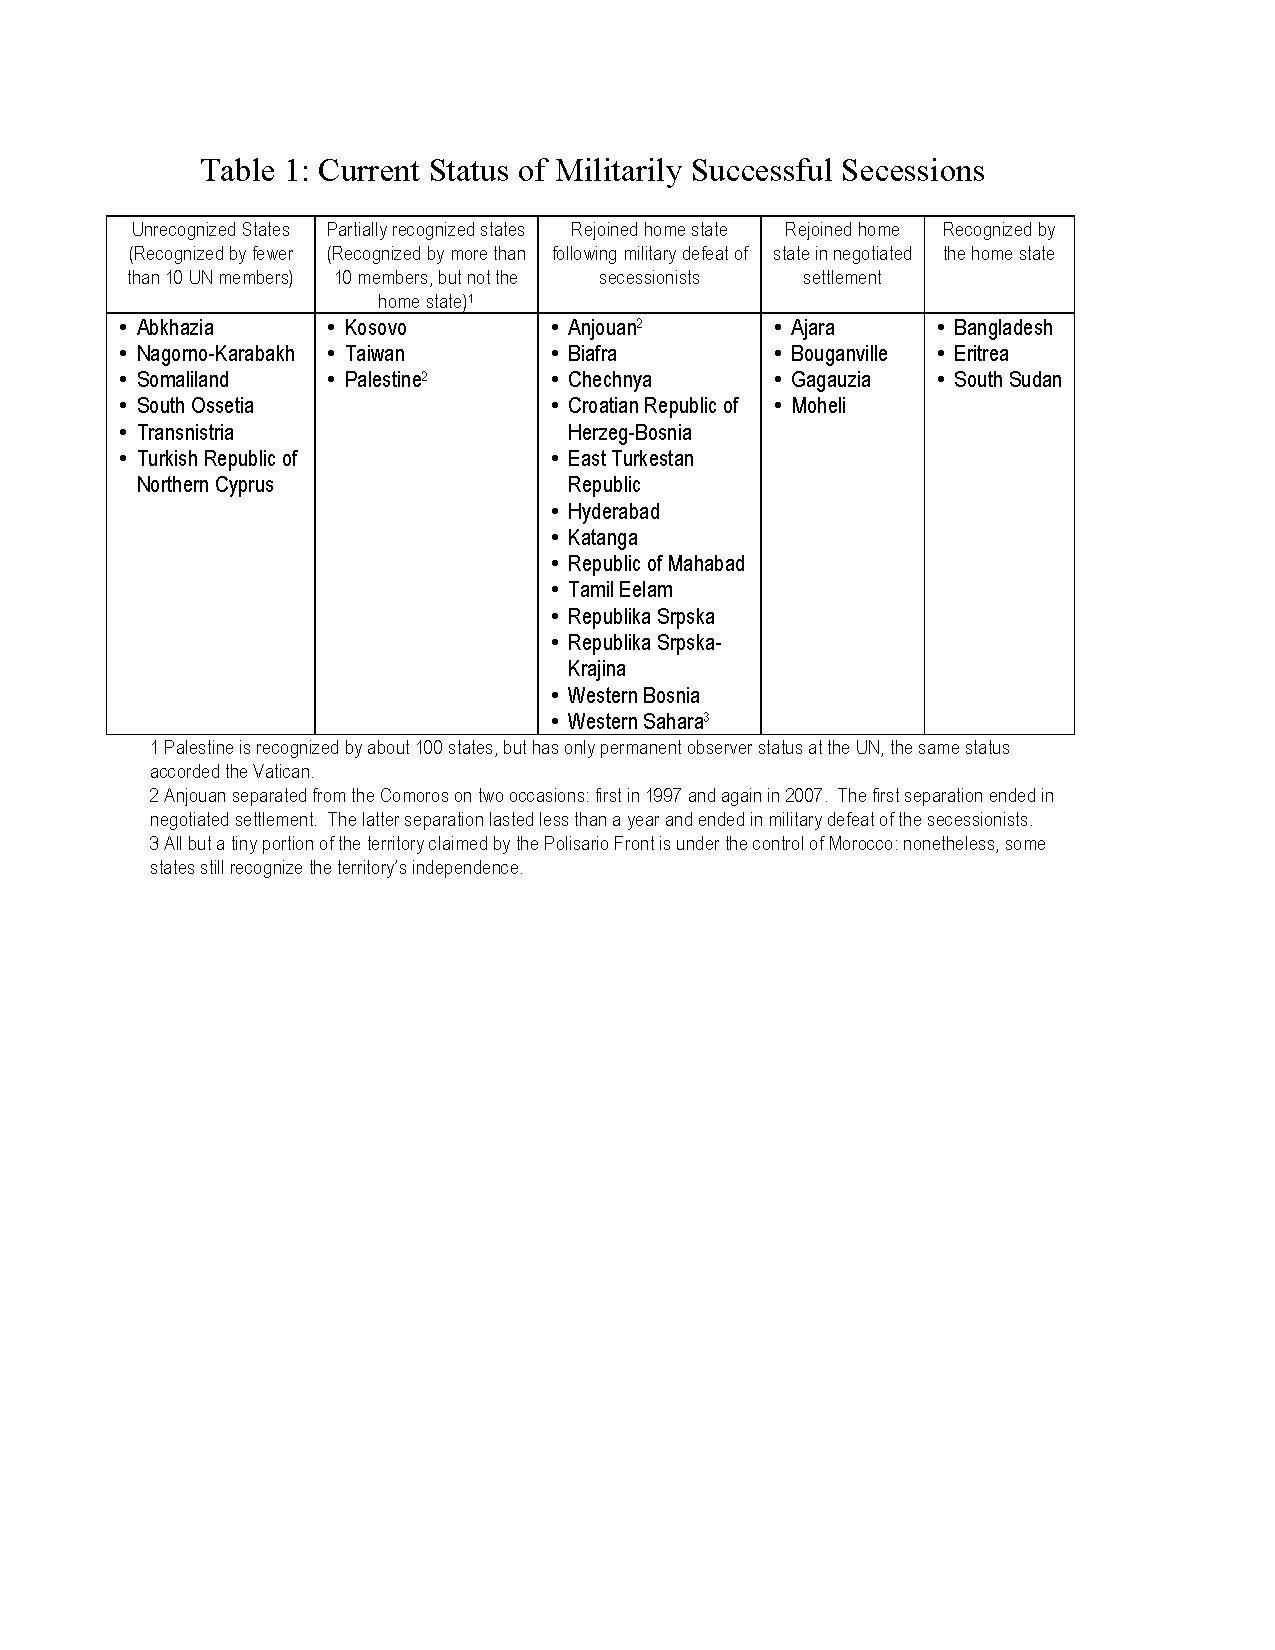
\includegraphics[width=6.25in]{Table_1_082214.pdf}
\end{center}

Of those cases in the table, all but Moheli controlled territory and govern(ed) populations for at least two years. These cases represent the most successful cases of attempted secession in the Post-WWII era, and yet eventual military defeat by the home state is still the modal form of resolution. Recognition by the home state is similarly rare, occurring in only three cases and never except as a direct result of concessions won on the battlefield. In cases where recognition by the home state or the right to a referendum on independence is not secured as part of the initial peace agreement, it has not historically been forthcoming. Only four cases of negotiated reunification are observed: secessionists who are strong enough to secure and retain territorial control are rarely willing to surrender their independence at the bargaining table, even though the chances of eventual recognition are vanishingly slim. Thus, the number of long-running, costly stalemates has been substantial, most of them eventually ending in military reconquest by the home state.

\subsection{Unrecognized States in the Literature}
%Political scientists care a great deal about both civil conflict and about state formation, but unrecognized states do not sit neatly in either literature. The literature on civil war is focused primarily on war onset (e.g. Fearon and Laitin 2003; Hegre and Sambanis 2006), war intensity and duration (e.g. Collier and Hoeffler 2004; Cunningham 2006), and the durability of post-conflict peace (e.g. Hartzell, Hoddie and Rothchild 2001). Unrecognized statehood does not fit neatly into these areas of study because, while unrecognized states begin, and often end, through violent conflict, periods of unrecognized statehood generally contain little, if any, fighting. %Unrecognized statehood often represents a relatively stable end to civil war, but the cessation of fighting is not coterminous with resolution of the conflict in any meaningful way. We argue that persistent unrecognized statehood is not a successful resolution to secessionist civil war; it is a costly and normatively bad outcome in its own right, and it needs to be analyzed as such. 
%Unrecognized states also fall outside most treatments of state formation, because most unrecognized states never achieve recognition (or have not achieved it yet).\footnote{For example, Roeder (2007) treats unrecognized states simply as failures to gain recognized statehood, not as outcomes to be analyzed in their own right.} 

The political science literature on civil war is focused primarily on war onset, %\footnote{e.g. Fearon and Laitin 2003, Hegre and Sambanis 2006}
war intensity and duration, %\footnote{e.g. Collier and Hoeffler 2004; Cunningham 2006} 
and the durability of post-conflict peace. %\footnote{e.g. Hartzell, Hoddie and Rothchild 2001} 
Unrecognized statehood does not fit neatly into these areas of study because, while unrecognized states begin, and often end, through violent conflict, periods of unrecognized statehood generally contain little, if any, fighting. Unrecognized states also fall outside most treatments of state formation, because most unrecognized states never achieve recognition (or have not achieved it yet).\footnote{For example, Roeder (2007) treats unrecognized states simply as failures to gain recognized statehood, not as outcomes to be analyzed in their own right.}  

The first literature to address unrecognized states directly was grounded in comparative politics, and a robust area-studies literature exists around each of the current cases of unrecognized statehood.\footnote{Lynch (2004), King (2001), Stanislawski (2008), and Bakke et al. (2013) provide notable treatments of the Former Soviet cases, and a pair of edited volumes by Bahcheli, Bartmann, and Srebrnik (2004) and Kingston and Spears (2004) each compile broader sets of case studies.} More recent literature has addressed wider ranges of cases and made important conceptual progress identifying patterns and commonalities across cases (e.g. Pegg 1998; Kolst\o \ 2006; Geldenhuys 2009; Caspersen and Stansfield 2011; Caspersen 2013). Bakke (2011) summarizes four explanations for the persistence of unrecognized states, each of which plays a role in the theory we develop here. First, economic and political elites benefit from the status quo (e.g. King 2001). Second, the secessionists have sufficient military capacity to make military reconquest costly (e.g. Kolst\o \ 2006). Third, secessionists enjoy external support from a patron (e.g. Lynch 2002; Stanislawski 2008. Lastly, the governments of unrecognized states are internally legitimate, enjoying support from residents of the unrecognized state (e.g. Lynch 2002, Kolst\o \ 2006).

However, the literature continues to lack a clear general theory specifying the conditions under which this outcome emerges and persists. 

One of the major contributions of this article is to provide a unified analytic framework for understanding the mechanisms sustaining unrecognized statehood as a stable equilibrium. By modeling unrecognized statehood formally, we move away from a case-by-case treatment toward development of a rigorous general theory. The model allows us to assess the conditions under which unrecognized statehood persists, and those under which war and negotiated settlement occur. It also allows us to evaluate various strategies available to actors, particularly states and coalitions of states who want to facilitate a peaceful and permanent resolution.

Although we are not aware of any formal models of unrecognized statehood there is a growing economics literature that employs game theoretic models of conflict. An early model of territorial disputes in which the divisibility of the contested territory is an important parameter is Grossman (2004). In Hirschleifer, Boldrin and Levin (2009), conflict can be avoided when there is common knowledge, a common rate of time preference, and players can make a series of small concessions. In our context, the contested territory is indivisible; this implies that peace would require very large concessions so that this pathway of using small compromises to avoid conflict is not available.

In contrast to Bueno de Mesquita (2013), which exemplifies a class of literature that examines how rebel groups make decisions about resistance strategies, we begin our analysis at the point where initial rebellion has already been successful to the point of gaining \textit{de facto} control of the disputed territory.

Another strand of the literature explicitly models the bargaining process between potential adversaries, either with asymmetric (Yared 2010) or complete information (Jackson and Morelli 2007, Schwartz and Sonin 2008, Bevi\'{a} and Corch\'{o}n 2010, McBride and Skaperdas 2014). Acemoglu, Golosov, Tsyvinski and Yared (2012) develop a dynamic model of resource wars featuring limited commitment. We abstract from questions of resource allocation and bargaining in order to focus on the dynamics created by the involvement of outside players: in the case of unrecognized states, the international community and patron states.

We next turn to presenting the model. In Section 3, we present a set of conditions under which unrecognized statehood is a stable, long-run equilibrium outcome. In Section 4, we analyze the potential effects of sanctions on the resolution of territorial disputes while Section 5 explores extensions of the model. Section 6 evaluates policy implications of the model, assessing various strategies available to outside actors that seek to induce their preferred outcomes. Section 7 concludes.


\section{A Model of Unrecognized Statehood} 
We model a dispute over a piece of territory that is controlled by a secessionist group and also claimed by a home state. The central issue of contention, independence vs. reunification, is both difficult to divide and highly valued by both sides. The secessionists seek recognized statehood, the home state seeks reunification, and these demands do not vary over time. The side payments that can be offered in exchange for the opponent's surrender of the independence/reunification issue are sharply limited by the absence of large concessions that can credibly be made (Walter 1997, 2002; Schultz 2010).

A major innovation of our model is the introduction of international actors. While the role of outside actors in determining the duration and outcome of civil conflicts is well documented (e.g., Elbadawi and Sambanis 2000; Regan 2002; Balch-Lindsay, Enterline, and Joyce 2008), the role of these actors has not been incorporated into the modeling of these conflicts.\footnote{One exception is van Houten (1998), who models the patron state ("reference state'') as a player in ethnic conflicts but otherwise takes an approach quite different from ours.} This is true even of work that addresses the role of outside actors as potential third-party enforcers (Walter 1997, 2002).

The model presented here allows us to both articulate the mechanisms that create these persistent stalemates and to assess the consequences, intended and otherwise, of outside actors' attempts to foster their desired outcome.\footnote{For another example of the strategic manipulation of decision-makers into (and out of) conflict see Baliga and Sjostrom (2012).}

\subsection{The Players}

We construct a model with four players: the secessionist elite ($s$); the central government of the home state ($g$) from which $s$ is attempting to secede; and two other players, the patron ($p$) and the international community ($c$). The latter two are outside actors---states, groups of states and/or individuals acting in concert---that have interests in the outcome of the attempted secession.

Player $c$ prefers reunification to recognized independence---a preference that is common to most states, and especially among those that fear the prospect of secessionist movements within their own borders. As discussed earlier, most states in the international system prefer any given secessionist conflict to be resolved by reunification. In practice we believe that in most cases there are many states that may act as player $c$ in our model, and often we observe groups of states like the OECD or the UN acting in this capacity. Modeling the international community as a single actor is a strong simplifying assumption, but by leaving the preferences of player $c$ quite general, the model can accommodate much of this diversity.\footnote{A variety of scholars, including Owtram (2011) and Coggins (2011) discuss the international relations of unrecognized states and variation across third-party states in their preferences with regard to unrecognized states.}

Player $p$ most prefers recognized independence, aligning its interests with the secessionists. We refer to $p$ as the patron because $p$ contributes resources to the unrecognized state in the status quo equilibrium. Patrons choose to contribute resources to secessionists for one or more of several reasons: 1) As an efficient mechanism for imposing costs on the home state (Salehyan, Gleditsch and Cunningham 2012), e.g. as Russia does to Georgia via South Ossetia and Abkhazia; 2) ethnic solidarity with the secessionists (e.g. Turkey's support of the Turkish Republic of Northern Cyprus); 3) hope of eventual annexation of the disputed territory (e.g. Armenia's support of Nagorno-Karabakh).\footnote{While annexation is appealing to many patrons (and some unrecognized states), annexation is not an outcome we model. International norms against irredentism are strong, and the costs of annexing an unrecognized state appear to be prohibitively large in most cases (e.g. Zacher 2001). Prior to Russia's annexation of Crimea, all post-WWII cases of annexation involved the annexation of colonial territory, rather than parts of the metropole. Israel's occupation of the Golan Heights and the West Bank are possible exceptions here.}

We acknowledge that there may exist patrons whose most-preferred outcome is the status quo. This naturally makes a status quo equilibrium easier to achieve, as there is an actor who strictly prefers the status quo and can expend resources to make it more likely. We choose to examine the case where the patron's most preferred outcome is independence because this is the condition under which the status quo is least likely. Even in this circumstance, the status quo remains an equilibrium outcome.    

\subsection{Timing and Structure of Interaction}

The game begins at a status quo in which the secessionist elite controls at least some of the disputed territory, but cannot gain international recognition unless the central government cedes its claim to the territory. This condition is archetypical of cases in which a militarily successful war of secession ends in a ceasefire.  

The payoff functions and all parameters, including probabilities in the war lottery, are common knowledge for all players, and actions are immediately observed by all players at the time they occur. There are an infinite number of periods $t=1,2,\ldots$, with play proceeding until an absorbing state is reached.

Future payoffs are discounted with a common parameter $\de$, where 1/$\de$ is each player's discount rate and $0\leq\de\leq1$.\footnote{All of the results that follow go through essentially unchanged in the general case where the players potentially discount at different rates. This simplifying assumption is made solely to highlight the essential mechanisms of the model.} Therefore payoffs for the entire game for player $i\in \{s, g, p, c\} $ can be expressed by the discounted stream of payments $\Sigma_{t=1}^{\infty} U_{it} \de^{t-1}$. 

In each period, play proceeds as follows:

\begin{figure}
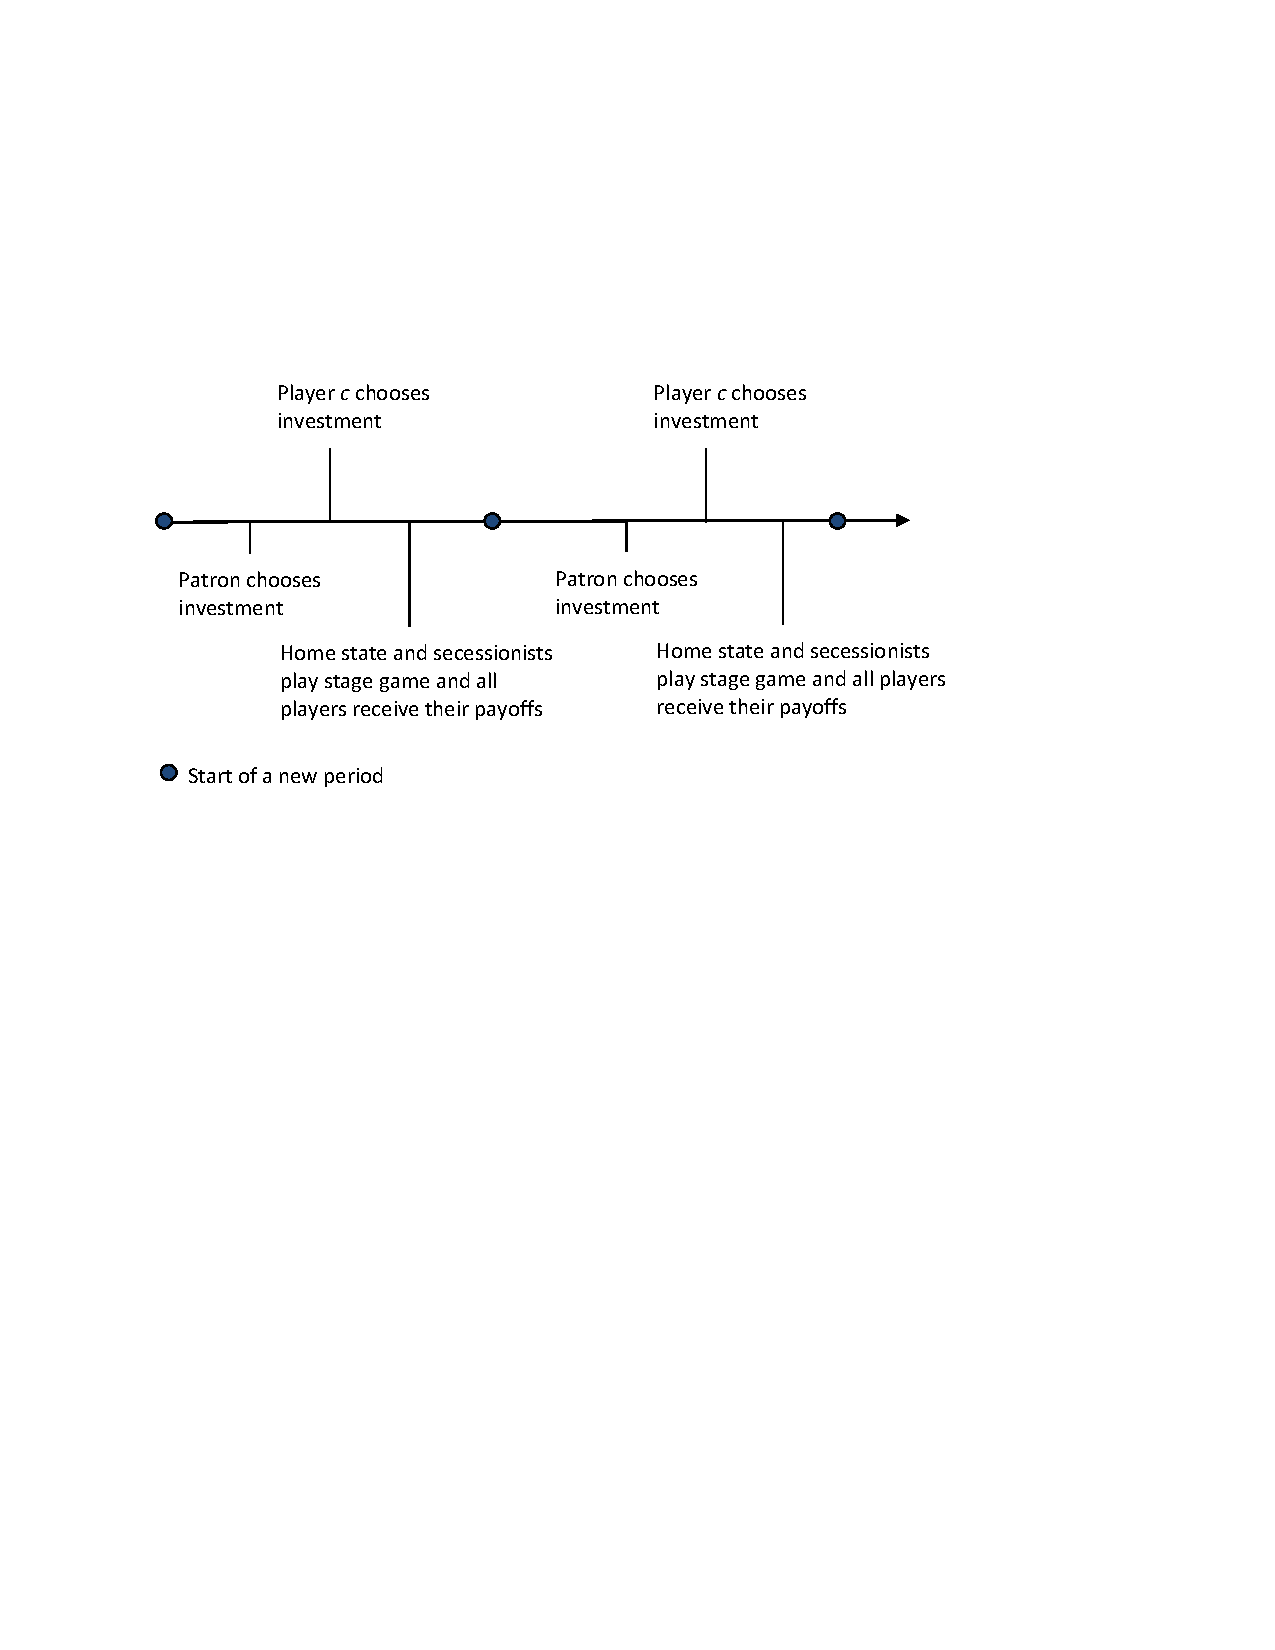
\includegraphics{Timeline2.pdf}
\caption{Timeline}
\end{figure}

\begin{enumerate} 
\item The status quo payoffs for $s$ are reduced by $\mu$.

\item $p$ chooses a level of resource expenditure $R_{pt}\in \mathbb{R}^+$ in period $t$ and invests it to alter the payoffs of players $s$ and/or $g$. 
 
\item $c$ chooses a level of resource expenditure $R_{ct}\in \mathbb{R}^+$ in period $t$ and invests it to alter the payoffs of players $s$ and/or $g$. 
 
\item $s$ and $g$ play a stage game in which each chooses simultaneously from the following actions: $\{\text{Fight, Status Quo, Cede}\}$. 
\end{enumerate}

In order to fully describe the structure of the game, we first introduce the stage game payoffs.

\subsubsection{Stage Game Payoffs}

\noindent Stage game payoffs for players $s$ and $g$ in period $n$, gross of investments by players $p$ and $c$, are:
\vspace{2pt}
\begin{center}
\begin{tabular}{|  c| c | c | c |} 
\hline
  $g\downarrow$,     $ s\rightarrow$  & Fight & Status Quo &Cede \\ \hline
	Fight & $\Omega_t$ &$\Omega_t$&$W_{gt}, L_{st}$ \\ \hline
	Status Quo& $\Omega_t$& $Q_{gt}, Q_{st}$ &$W_{gt}, L_{st}$ \\ \hline
	Cede&$L_{gt}, W_{st}$& $L_{gt}, W_{st}$ &$Q_{gt}, Q_{st}$ \\ \hline
 \multicolumn{4}{c} {Figure 2: Stage Game Payoffs}\\ 
\end{tabular}
\end{center}
\vspace{2.5pt}

If either $s$ or $g$ plays Cede while the other plays Fight or Status Quo, the game enters an absorbing state (i.e. the game ends), with payoffs in every subsequent period given by the corresponding entry in the stage game (Figure 2). We interpret one player ceding as that player ceding the issue of status (independence vs. reunification) in exchange for some set of (relatively small) payments from the opposing player. For example, if the secessionists cede, the secessionist region is reunified with the home state and the payoffs are $L_s$ for the secessionists and $W_g$ for the home state. Therefore, if one player agrees to cede while the other player chooses to remain in the status quo or fight, the result is a negotiated settlement benefiting the player who did not cede. 

If both states simultaneously play Cede, we assume that both renege immediately and that the status quo is preserved for that period. In this case neither player has demonstrated a willingness to give up more than the other. Therefore, payoffs for both players ceding simultaneously are identical to the status quo payoffs.%\footnote{This assumption is appropriate as precise simultaneity is an artifact of discrete time modeling: it is not a phenomenon we observe in the real world.} 

There are three ways to end up in war: either of the parties may attack first, or both may attack simultaneously. We denote the payoffs of war as a lottery $\Omega$.\footnote{Because the unrecognized state already controls territory and the \emph{de facto} borders are armed, there is likely only a small advantage to be gained by attacking first for either side. Therefore, we argue it is not essential to differentiate between these war scenarios analytically.} This lottery determines whether the secessionists or government wins the war. For simplicity, we assume the outcome of the war is an absorbing state.\footnote{The model can easily be extended to encompass the possibility of an indecisive war.} Outright victory would, among other things, allow an unrecognized state to force recognition by the home state government. Therefore, outright victory requires more than simply securing control of the disputed territory (which the secessionists have already done when the game begins) and requires the ability to impose the terms of settlement. In practice, this likely involves the capture of the home state capital and/or the overthrow of the home state government.

For probabilities $p_1$ of outright victory and $1-p_1$ of loss, player $i \in \{s, g\}$ in period $t$ with a fixed cost of war $\zeta_i$ faces war lottery $\omega_{it} \equiv (p_1 (W_{it}-\zeta_i), \left(1-p_1\right)( L_{it}-\zeta_i))$. $\Omega_t \equiv (\omega_{gt}, \omega_{st}).$\footnote{Baseline costs of war are fixed ($\zeta_i$) but additional costs of war based on war's result are captured in $W_i$ and $L_i$.} Players are assumed to approach war lotteries as expected values.

If both $s$ and $g$ play Status Quo, then the status quo persists. The status quo payoffs for the secessionists are modeled as a state variable. The transition of this state variable from one period to the next involves an increase by the amount of the patron's investment and an automatic reduction by $\mu$.\footnote{Note that it is also possible for the international community to make an investment in the secessionists' status quo payoffs, but we will show that they have no incentive to do so.} The steady reduction by $\mu$ represents the costs of non-recognition discussed in the introduction. As the economy in the secessionist region deteriorates, so does the standard of living for the secessionists. Therefore, the payoffs from the status quo, in the absence of other actions, are given by $q_{s,t+1} = Q_{s,t} - \mu$. Lower case letters denote beginning-of-period quantities net of investments by outside actors, while upper case letters denote end-of-period quantities gross of such investments.

Other payoffs are also modeled as state variables. However, they remain unchanged from period to period unless players $p$ or $c$ make an investment, e.g. $L_{s,t} = l_{s,t} + R_{p,t} + R_{c,t}$ and $l_{s,t+1} = L_{s,t}$, likewise for player $g$ and for the payoffs from winning for both players and the status quo for player $g$. 


\subsubsection{Payoffs for the Patron and International Community}

At the start of each period, the patron, $p$, and player $c$ may invest resources to affect the payoffs of $s$ and $g$ in the stage game. For example, if $p$ expends resources $R_{pt}$ to increase the secessionists status quo payoffs, the beginning-of-period payoff $q_{st}$ becomes end-of-period payoff $Q_{st} = q_{st} + R_{pt}$. We can write analogous expressions for $q_{gt}, \ l_{st},\ l_{gt},\ w_{st}$, and $w_{st}$, and the international community can also make investments to increase whichever of these payoffs they like. $B_{pt}$ denotes the total that the patron can devote to interceding in the conflict; we assume that player $c$, which is often a large coalition of states, does not have a binding budget constraint.

We assume player $c$ prefers peace to war. For simplicity, we limit our modeling of $c$'s preference for peace to the assumption that $c$ will not choose to fund a military buildup that it expects will induce war. This assumption is not necessary for the basic results to hold; however, it justifies our decision not to address military support of armed reconquest by the home state as a deliberate strategy by $c$ to achieve reunification. 

We use two binary variables to express the preferences among the three outcomes (status quo, reunification, recognition by the home state) for both $p$ and $c$. $X$ is a binary variable representing reunification: $X=0$ in the status quo and $X=1$ if the secessionists rejoin the home state. Y represents recognition by the home state of the secessionists' independence: $Y=1$ if the home state recognizes the secessionists as independent, $Y=0$ otherwise. 

Player $p$'s payoffs in period $t$ are $U_{pt}= -\alpha X+\lambda Y -R_{pt}$, while the payoffs for player $c$ are $U_{ct}= \beta X-\nu Y -R_{ct}$, with both payoffs denoted in currency units. Taking $\alpha, \ \beta, \lambda,$ and $\nu$ to be positive, these payoffs represent the idea that the patron opposes reunification while player $c$ prefers it, and that the patron prefers recognized independence while player $c$ is averse to the creation of new states.

The relative strengths of the patron and player $c$'s preferences determine their willingness to spend resources. As we will show, unrecognized statehood emerges as an unhappy but stable middle ground in which all players avoid their least preferred outcomes.

%While in many cases both the central government and the de facto government of the unrecognized states may be relatively autocratic, leaders still rely on some level of public support to remain in power.  If the leaders' actions deviate too far from the public's preferred course, they may be removed from office or forced to bear the costs of additional repression of regime opponents.  Therefore, both the central government and the secessionist elite have incentives to take the public's opinions into account, and the preferences of the public are thus internalized in the payoffs expressed in the model for $c$ and $g$. 

\subsubsection{The Low Payoffs from Ceding}
Aside from the central assumption that the government of the home state most prefers reunification and the secessionists most prefer independence accompanied by international recognition, we will for the most part leave the model general enough to incorporate a range of preferences and capabilities for players $g$ and $s$. %Our results will specify parameter ranges for these preferences over which outcomes of interest---such as perpetual unrecognized statehood---can be supported in equilibrium.
We do, however, assert that the payoffs for the party that cedes the issue of status (independence vs. reunification) are consistently low. This reflects a combination of two factors. First, the issue of status is indivisible\footnote{Either the unrecognized state has sovereignty over its territory and is co-equal with the home state, or the secessionist region (and its government) are subordinate to the central government.} and highly valued by each side, making its surrender undesirable. Various forms of ethno-nationalism often motivate secession, and the values attached to independence by secessionists (and to reunification by citizens of the home state) are generally large relative to the values placed on economic prosperity and other goals. Second, many of the payments that could be offered are not credible (e.g. Schultz 2010).

The difficulty of making credible payments in exchange for status is one clearly demonstrated in the civil war literature (e.g. Licklider 1995; Walter 1997, 2002; Fearon and Laitin 2007; Doyle and Sambanis 2006). Unrecognized states generally constitute ``sons of the soil" conflicts in which the central government cannot credibly commit to preserving the local demographic and political dominance of the secessionist elite once the disputed territory reverts to central government control (Weimer 1978; Fearon 2004). While the central government might initially grant the secessionist elite a high level of autonomy in exchange for agreeing to reunification, the level of autonomy is likely to decrease over time, perhaps quite quickly. The payments that can be offered by the unrecognized state to the central government are similarly small or unenforceable: once recognition is achieved, the secessionists have little reason to uphold any prior commitments. 

%At the time of secession, ethnic Akbhaz made up a minority of the population of Abkhazia, but by the late 1990s they controlled almost all political posts in the \textit{de facto} government of the region (Cornell 2001; Wooleh 2006). In 2004, the basket of payments offered by the Georgians in exchange for reunification included a provision guaranteeing that ethnic Abkhaz would retain a majority in the regional parliament, even if the return of internally displaced persons (IDPs) once again placed ethnic Abkhaz in a minority demographic position in the region. The promise, however, was not very meaningful. First, even if the promise were upheld, it would still mean a step back from the total dominance the ethnic Abkhaz currently enjoy in the region. Second, if Georgian IDPs returned, they may demand and receive a more equitable system of representation. These concerns are not abstract; this type of reneging has already occurred in cases that did reach settlement.

The case of Gagauzia illustrates the commitment problem nicely. Gagauzia achieved \emph{de facto} independence at the time of the Soviet Union's collapse, but agreed to rejoin Moldova in 1994 as an autonomous region. While Gagauzia was granted substantial autonomy under the Moldovan Law on the Special Legal Status of Gagauzia, when the governor of Gagauzia, Dmitrii Croiter, moved to assert these powers in 1999, the Moldovan government balked. By 2002, Croiter was forced to resign, effectively deposed by the Moldovan government. The Moldovan government jailed a number of other Gagauz politicians, and while \emph{de jure} Gagauz autonomy was enshrined in the Moldovan constitution in 2003, the \emph{de facto} level of autonomy has been limited by continued central government meddling in less-than-free regional elections. The payoffs to Gagauzia for ceding have turned out to be quite low, and a similar fate can rationally be expected by other unrecognized states who choose to cede.
%WE CAN CUT THE GAGAUZ EXAMPLE IF NECESSARY -- BG July 2014


%The payments that can be offered by the unrecognized state to the central government are similarly small or unenforceable. To return to the Abkhaz example: Under a scenario in which Georgia recognizes Abkhazia as an independent state, the ethnically Georgian region of Gali, currently under Abkhaz control, would likely rejoin Georgia, Russian troops would be (at least temporarily) expelled, and compensation might be paid to displaced Georgians, but other side payments are difficult to picture. Abkhazia might promise Georgia privileged access to Abkhaz ports, or promise to keep Russian troops out of its territory permanently, but once recognition is granted, any such promises could easily be reneged upon.

%Furthermore, while relinquishing territorial claims relieves the home state of a persistent source of instability, conceivably supplementing $g$'s payoffs from ceding, it also would increase the probability of future attempts at secession by other regions (Walter 2006). The lack of enforceable side payments and the ambiguous impact on stability make ceding the issue of status a low-payoff option for $g$, just as it is for $s$.

%Among the means through which $p$ or $c$ can spend resources to alter the payoffs to $g$ and $s$ is to enforce bargains and guarantee future concessions by either party, raising the payoffs from ceding. For example, if both the home state and the secessionists prefer reunification with autonomy rights to both war and continued stalemate, $c$ can spend resources to enforce an agreement in which the secessionists are promised specific autonomy rights and $c$ agrees to ensure that these rights are later retained. Should the home state later attempt to revoke the promised autonomy, $c$ can levee sanctions or employ other coercive measures to deter this action. The promises and pitfalls of this approach are discussed in the section on policy implications of the model.

\section{Explaining Outcomes of Secessionist Conflicts} 
\label{sec:main}
%The game has three outcomes that we will consider, each of which can be characterized by a class of equilibria. The outcome of greatest interest is both players choosing the status quo in perpetuity; we will also examine the two absorbing states, reunification and recognition by the home state (i.e. recognized statehood).\footnote{Other classes of equilibria are possible, for example it is theoretically possible for the players to agree to a lottery between the absorbing states which would yield a higher expected payoff than the status quo. However, in practice there is a credibility issue: the losing party does not have an incentive to cede if they lose the lottery. Such strategies are, in any case, not analyzed here.} 

Despite the preferences of the international community for peace, the most common outcome of secessionist conflicts in the post-WWII period has been reunification with the home state via outright military reconquest. By contrast, reunification through negotiated settlement has been very rare. We will explore potential explanations for this seeming inability of the international community to achieve its aims in Sections~\ref{sec:alt} and \ref{sec:ext}. First, we turn to the outcome that we find the most puzzling: perpetual unrecognized statehood.

\subsection{Analysis of the ``Status Quo'' Equilibrium} 
\label{sec:mainproof}
Unrecognized states are frequently viewed as temporary phenomena or as non-equilibrium outcomes attributable to players' misperceptions of the strategic situation, or their fundamental irrationality. Our central result shows that unrecognized statehood can be an equilibrium outcome capable of being sustained in perpetuity by fully rational, perfectly informed actors. This is true even when there is no actor that prefers unrecognized statehood as a first-best outcome.

We begin by listing and providing intuition for a set of restrictions on the preferences of the actors and their resources for which we can guarantee that unrecognized statehood is an equilibrium outcome. This set of restrictions identifies a class of games, $\mathcal{G}$: 

\begin{definition}
\emph{The class $\mathcal{G}$ includes all those games for which the parameters satisfy the following restrictions:}

\begin{enumerate}
\item \textit{For both players $g$ and $s$, $Q_{i0} \geq L_{i0}$: remaining in the status quo is better than ceding at the beginning of the game.}

\item \emph{For both players $g$ and $s$, $\frac {Q_{i0}}{1-\delta} \geq  -\zeta_i+\frac{W_{i0}(p_{1i}) + L_{i0}(1-p_{1i})}{1-\delta}$: the expected outcome under war is worse than the status quo at the beginning of the game.}

\item \textit{$\frac{\alpha}{1-\de} \geq \frac{\beta}{1-\de} + \mu$: reunification is more important for the patron to avoid than for the international community to achieve.}

\item  \textit{$\nu\cdot p_{1s} \geq \lambda \cdot p_{1s} + \mu + \beta$: recognition of the secessionist state is more important for the international community to avoid than for the patron to achieve.}

\item  \textit{$B_{p1} \geq\frac{\beta}{1-\delta} - \left(Q_{s0} -\mu - L_{s0} \right)$: the patron can afford to deter player $c$ from inducing reunification at the beginning of the game.}

\item \textit{$B_{pt} \geq \mu, \ \forall t>1$: the patron can afford to pay to maintain the status quo.}\footnote{Depending on parameters, condition (5) is more likely to be binding than condition (6). If there is great variance in budget between periods for the patron, such as a greatly reduced budget in some period $t> 1$ compared to period $1$, (6) could be binding.}

\end{enumerate}
\end{definition}

There are many potential equilibrium outcomes of this game, including, under the right parameters, immediate ceding by either party as well as fighting (see Section~\ref{sec:alt}). As we are interested particularly in the outcome of long-term unrecognized statehood, here we focus on the question of the existence of an equilibrium that leads to this outcome in perpetuity. We will show that, given a game satisfying the parameter restrictions in Definition 1, at least one status quo equilibrium will exist.

Our concept of equilibrium will be stationary Markov equilibrium as defined in Mailath and Samuelson (2006). That is, a strategy profile is a stationary Markov equilibrium if it is a stationary Markov strategy profile and a subgame-perfect equilibrium. In turn, a strategy profile is defined to be a stationary Markov strategy if any two ex post histories terminating in the same state play identically from the termination point forward. That is, stationary Markov strategies ignore all details of the history aside from the current state.

The state is a vector of six variables comprised of the payoffs from the status quo, ceding, and winning the issue of status for each of the two inside actors. That is, $s = \left(q_s,q_g,l_s,l_g,w_s,w_g \right)$. Strategies for the patron and the international community are how much to invest in each of the six state variables. However, positive investments in some of the state variables can be ruled out by preference assumptions.

Player $c$ dislikes war and so will never invest in $w_s$ or $w_g$, which only serve to increase the likelihood that one of the inside actors chooses to fight. It would also not want to make the government lose and so won't invest in $l_g$. This leaves three state variables in which player $c$ might invest: $q_s$, $q_g$, $l_s$.

Because the patron's preferences are aligned with the secessionists and against the government, it never invests in $w_g$ or $l_s$. The only reason the patron would invest in $q_g$ is to counter an investment by player $c$ in the government's payoffs from war; since player $c$ will not make such an investment, we can also rule out investments by the patron in $q_g$. This leaves four state variables in which the patron may invest: $q_s$, $l_g$ and $w_s$.

In equilibrium, the outside actors' investments are paired: the patron investments in the secessionists' status quo payoffs deter player $c$'s investments in the secessionists' payoffs from ceding. Likewise, investments by player $c$ in the government's status quo payoffs deter the patron from investing in the government's payoffs from ceding. Investments by player $c$ in the secessionists' status quo payoffs deter the patron from investing in the secessionists' payoffs from winning the conflict via fighting. In each case, the investments are sufficient to make the largest continuation payoffs in the game between the secessionists and the government those from playing status quo.

\begin{definition}
The Status Quo Equilibrium is a stationary Markov equilibrium in which the outcome is perpetual unrecognized statehood. The strategy profiles are the following, organized according to the patron's investments in each state variable. In period $t$:

\begin{enumerate}
	\item The patron invests $R_{pt} = \max\left\{\frac{\beta}{1-\de} - \left( Q_{s,t-1} - \mu - L_{s,t-1}\right),0\right\}$ to augment $q_{st}$. Player $c$ invests $R_{ct} =0$ in $l_{st}$.

If $R_{pt} < \frac{\beta}{1-\de} - \left( Q_{s,t-1} - \mu - L_{s,t-1}\right)$ player $c$ invests $R_{ct} = l_{st} - \left(q_{st} + R_{pt} \right) + \ve$, for $\ve$ small, in $l_{st}$. Cede becomes the unique best response for the secessionists.

	\item As long as $R_{pt} \leq \frac{\nu}{1-\de} + \left( Q_{g,t-1} - L_{g,t-1}\right)$ to augment $l_{gt}$, player $c$ invests $R_{ct} = R_{pt} - \left( Q_{g,t-1} - L_{g,t-1}\right)$ in $q_{gt}$. Note that the outcome is that investments in $l_{gt}$ and $q_{gt}$ are zero.

If $R_{pt} > \frac{\nu}{1-\de} + \left( Q_{g,t-1} - L_{g,t-1}\right)$ to augment $l_{gt}$, player $c$ invests $R_{ct} = 0$. Cede becomes the unique best response for the government.

	\item As long as $R_{pt} \leq \frac{1}{p_{1s}} \left[\frac{\nu p_{1s} - \beta (1-p_{1s})}{1 -\de} - \mu + Q_{s,t-1} - \left(-\zeta_{s}(1-\de) + W_{s,t-1}p_{1s} + L_{s,t-1}(1-p_{1s})\right)\right]$ to augment $w_{s,t}$, player $c$ invests $R_{ct} = R_{pt}p_{1s} + \mu - Q_{s,t-1} + \left(-\zeta_{s}(1-\de) + W_{s,t-1}p_{1s} + L_{s,t-1}(1-p_{1s})\right)$ in $q_{st}$. Similar to case two, the outcome is that investments in $w_{st}$ and $q_{st}$ are zero.

If $R_{pt} > \frac{1}{p_{1s}}\left[\frac{\nu p_{1s} - \beta (1-p_{1s})}{1 -\de} - \mu + Q_{s,t-1} - \left(-\zeta_{s}(1-\de) + W_{s,t-1}p_{1s} + L_{s,t-1}(1-p_{1s})\right)\right] $ to augment $w_{s,t}$, player $c$ will choose $R_{ct}=0$. Fight becomes the unique best response for the secessionists.
\end{enumerate}
The government and secessionists play their best responses in the stage game given the continuation values induced by the investments of the outside actors. Unless otherwise noted above, playing Status Quo is the best response for both inside actors.
\end{definition}

\textbf{Need text to give intuition or tell where I'm going to give intuition.}

\begin{quotation}
\noindent \bf \emph{Proposition 1:} \rm  \emph{There exists an equilibrium in which the outcome is perpetual unrecognized statehood. The actions in this equilibrium are for $p$ to invest to create a buffer of $\frac{\beta}{1-\de}$ between the payoffs from ceding and the status quo in the first period and to invest up to $\mu$ each period thereafter to maintain the buffer; for $c$ to pay nothing; and for both $g$ and $s$ to play $Status$ $Quo$ each period.}


\end{quotation}

These conditions for the status quo are sufficient but not necessary. For example, if the status quo initially has a much higher long term payoff than the next best alternative for the secessionists, Condition (6) need not be met to maintain the status quo in the short run. The inequality \emph{will} bind for some set of periods $t \geq 1$ because the secessionist payoffs from the status quo decrease over time. In cases where condition (6) is not met, we can have unrecognized statehood for some time, but it is not a long-run equilibrium outcome.

\noindent {\bf Proof of Proposition 1} \\
Recall that each period is composed of three action stages: player $p$'s investment decision (stage 1), player $c$'s investment decision (stage 2), and the simultaneous game between players $g$ and $s$ (stage 3). Although period $t$ may be reached either because in period $t-1$ both players ceded or the status quo had been maintained, the strategic landscape in period $t$ is the same. Thus all periods in which the players are able to move are in an equivalence class in which the only possible strategic difference is in the value of the state variables.

Analysis of the posited equilibrium proceeds most naturally by backward induction within each period. Thus we begin with the stage game between the government and secessionists. We assume that the government and secessionists choose the Status Quo strategy whenever indifferent between it and any other strategy.

\begin{quotation}
\noindent \textit{{\bf Lemma 1:} $Q_{it} \geq L_{it}$ and $\frac {Q_{it}}{1-\delta} \geq  -\zeta_i+\frac{W_{it}(p_{1i}) + L_{it}(1-p_{1i})}{1-\delta}$ for $i \in \left\{g,s\right\}$ are sufficient for status quo to be the outcome of Stage 3 in period $t \ \forall t$.} 
\end{quotation}

The proofs of the lemmas are in the Appendix.

Lemma 1 establishes ranges for the payoffs for players $g$ and $s$---gross of investments by the outside players---in which the status quo outcome can occur. The rest of this section tackles the more difficult task of determining the incentives and actions of the outside actors---that is, the patron state and the international community---to impact those payoffs.

To begin, note that either outside actor could invest toward increasing any of the six state variables in a period: $q_{st},q_{gt},w_{st},w_{gt},l_{st},$ and $l_{gt}$.\footnote{In the case of $w_{st}$ and $w_{gt}$, it is more intuitive to imagine investments increasing the probability of winning a war; because the lottery is additively separable and the ``Win'' outcome is always preferred when it occurs independently in the stage game, this more convenient modeling choice is inconsequential.} It is not necessary to focus on which investment vehicle is optimal for a government to choose; what is essential is to determine which outcomes---i.e. \emph{Recognition, Status Quo}, or \emph{Reunification}---they will target given that they will choose the most efficient way to alter the payoffs of players $s$ and $g$.

%Given their preference orderings, some of these can be ruled out. Player $p$ will not invest to increase $s$'s payoffs from ceding ($l_{sn}$) or $g$'s payoffs from war when it could do so for $s$. It will also not invest in $q_{gn}$ when it can instead increase $l_{gn}$, leaving the list of rational investment choices for $p$ as $q_{sn},l_{gn}$, and $w_{sn}$. Symmetrically, $c$ will not invest in $q_{sn},L_{gn}$, or $w_{sn}$. Given the assumption that the international community follows a norm of encouraging peaceful resolution, it also will not invest in $w_{gn}$, leaving only $l_{sn}$ and $q_{gn}$ as rational investment options for player $c$.

Lemma 2 addresses potential efforts by the international community to influence the outcome toward \emph{Reunification}:

\begin{quotation}
\noindent \textit{{\bf Lemma 2:} When Condition 3 holds, the patron's willingness to invest to maintain the status quo is sufficient to deter the international community from intervening to encourage reunification.}
\end{quotation}

\noindent Condition 3 provides a bound on the amount that player $p$ must be \emph{willing} to invest each period in order to prevent player $c$ from contesting the status quo outcome. To complete the equilibrium construction, we must determine the utility maximizing investments by $p$ and conditions to ensure that it is \emph{able} to make those investments.\footnote{Efforts by the patron to create the conditions for the \emph{Recognition} outcome are addressed in Lemma 3 once the equilibrium investments are established.}

Consider period 1. When Condition (4) holds, the patron will want to invest just enough to create a buffer of $\frac{\beta}{1-\de}$ between $Q_{s1} \ (= q_{s1} + R_{s1})$ and $l_{s1}$ so that $c$ will not invest. That is, in equilibrium, $R_{p1} = \frac{\beta}{1-\de} -(q_{s1} - l_{s1})$ as long as $p$ can afford to make this investment. Thus we need Condition (5): $B_{p1} \geq\frac{\beta}{1-\de} - \left(q_{s1} - l_{s1} \right)$, where $B_{p1}$ is the amount $p$ has available to spend on the conflict in period $1$.

In periods $t > 1$, there are two cases to consider. Either (a) the buffer created in period $t-1$ was precisely the necessary $\frac{\beta}{1-\de}$, or (b) the buffer is larger than $\frac{\beta}{1-\de}$. In case (a), the patron must spend exactly $\mu$ to offset the degradation in the status quo payoffs and re-establish the buffer of $\frac{\beta}{1-\de}$.\footnote{A third case in which the buffer is smaller than $\frac{\beta}{1-\de}$ provides lower welfare to player $p$. Conditions (3) and (5) ensure that player $p$ can avoid this case.} In case (b), the patron can spend less than $\mu$ in period $t$. However, because in each period $q_{st}$ degrades by $\mu$, eventually the buffer will be reached and we will be returned to case (a). Again, assuming Condition (3) holds, the patron will want to make this investment if its budget allows, and so a sufficient condition is that $p$'s budget is at least as large as $\mu$ in every period $t > 1$ (Condition 6). 

With the equilibrium status quo investments determined, we can proceed to Lemma 3, which rules out spending for or against recognition of the secessionist state:

\begin{quotation}
\noindent \textit{{\bf Lemma 3:} When Condition 4 holds, the international community's willingness to invest to avoid recognition of the secessionist state is sufficient to deter the patron from investing to achieve recognition.}
\end{quotation}

In the equilibrium under consideration here, the patron will invest to maintain an outcome that is not its most preferred, but it will not invest to achieve its most preferred outcome. This behavior may appear counterintuitive, but we frequently observe patron states whose preferred outcomes are recognized independence for the secessionists who  nonetheless contribute resources to sustain a status-quo outcome that is costly to all involved. The patron does not attempt to contribute sufficient resources to force recognition by the home state because doing so would induce offsetting expenditures by the international community to prevent this outcome.\footnote{We do not provide conditions on the budget of player $c$ similar to Conditions (5) and (6): since the size of the international community relative to any particular country is large, it can be assumed that a budget constraint does not bind.}

One last possibility is ruled out by Lemma 4: that the patron would invest to encourage the secessionists to fight. 

\begin{quotation}
\noindent \textit{{\bf Lemma 4:} Conditions 3 and 4 ensure that the international community's willingness to invest to discourage new conflict is sufficient to deter the patron from investing to instigate such fighting.}
\end{quotation}

Note that this result depends on an implicit assumption that the patron is not able to skew the odds of the secessionists winning the conflict in a way that cannot be nullified by the international community. All other conflict scenarios are ruled out by the international community's assumed preference to avoid conflict.

Thus, given Conditions (1)-(6) hold, equilibrium strategies for each period in this status quo equilibrium are:
\begin{itemize}
	\item Player $p$ spends more than $c$ is willing to invest to ensure the incentives for the status quo outcome are in place in period $t$ whenever this is affordable. That is, $p$ invests $R_{pt} = \max\left\{0,\frac{\beta}{1-\delta} -(q_{st} - l_{st})\right\}\leq B_{pt}$. If this inequality is violated, $p$ invests nothing.
	\item Player $c$ invests $R_{ct} = \frac{\beta}{1-\delta} -(Q_{st} - l_{st})$ if $\frac{\beta}{1-\delta} > (Q_{st} - l_{st})$. Otherwise, it invests nothing. 
	\item Players $s$ and $g$ play Status Quo as long as it yields the highest continuation value, and play Cede or Fight if continuation values from either exceeds the status quo continuation value. 
\end{itemize}

Equilibrium actions are for $p$ to maintain the status quo by investing $\mu$ each period once the difference in payoffs to $s$ from playing Status Quo and Cede reaches $\frac{\beta}{1-\de}$ (with a possible lump sum investment at $t=1$ of up to that amount); for $c$ to not invest and for both $g$ and $s$ to play Status Quo each period. \hfill $\blacksquare$

%Our status quo equilibrium requires that $p$ invests in every period enough to maintain $F^*$ by offsetting the $\mu$ decline in the secessionists' status quo payoffs. The total per-period equilibrium investment $R_{pn}$, a flow payment, in the long run is thus $\mu$ per period in this steady state. In a status quo equilibrium $c$ need not invest at all since stage game payoffs of $g$ do not deteriorate.\footnote{ In the absence of the assumption in the model setup above that player $c$ does not want war, the patron would need to retain a second buffer against $c$ funding war.  The expected value of war for the home state would need to be maintained at a level lower than the status quo payoff by a buffer of $F*=\frac{\beta}{1-\delta_c}$. If this buffer did not exist in the first round of the game, the patron would fund the alteration of payoffs to create the buffer, thus assuring payments by $c$ would be ineffective at trying to change the home state's payoffs to make war more attractive than the status quo.}

By contributing $\mu$ in each period, the patron supplies sufficient resources to the unrecognized state to ensure that the secessionist elite prefers the status quo to surrendering independence. 

\subsection{Discussion}

The existence and durability of this not-infrequently observed status quo equilibrium is counterintuitive on two levels. First, the large, relatively rich international community is outspent by a relatively small, less-resourced patron; second, unrecognized statehood is a stable equilibrium in spite of being undesirable to all players. The key condition leading to this outcome is that each outside actor's willingness to pay to achieve its most preferred outcome is outweighed by the other's desire to avoid it's least desired outcome. An ongoing unresolved conflict results.

Despite its high costs, this equilibrium is quite robust. Because player $c$ and the patron can adjust contributions to reflect changing conditions on the ground, exogenous shocks that might otherwise have the potential to alter the equilibrium have their strategic impact nullified. For example, while a drought in the unrecognized state might decrease the secessionist elite's payoffs from the status quo and increase their need for international trade and assistance, additional humanitarian and economic assistance from the patron can offset the effects of the shock and preserve the status quo. Likewise, if the home state gains military strength, altering the probabilities in the war lottery, the patron can offset these changes by providing arms or otherwise investing in the defenses of the unrecognized state. See further discussion along these lines in Section~\ref{sec:sanctions}.

While we do not model this directly, the stability of the status quo equilibrium may be further enhanced by the reluctance of the patron to withdraw support for an unrecognized state that was previously supported. Fearon (1994) and subsequent work on audience costs suggests that, past a certain threshold of escalation, it becomes difficult for leaders to back down from confrontation because they fear looking weak in front of domestic audiences. Leaders of patrons that have supported the secessionists in a previous period may risk losing office if they later back down -- even if it is the best interest of the patron state to do so.  

\subsection{Alternative Outcomes}
\label{sec:alt}

The conditions of Proposition 1 \emph{do not} provide for a unique equilibrium, or even a unique equilibrium outcome. In fact, at least one additional equilibrium outcome always coexists with the status quo outcome.

If the payoffs from Fight are strictly greater than the payoffs from Cede for both players, then (Fight,Fight) will be the only additional equilibrium outcome. If this inequality holds for just one player, then we have only the additional outcome in which that player chooses Fight and its opponent cedes. If both players strictly prefer Cede to Fight, then both the (Fight, Cede) and (Cede,Fight) outcomes are added to the status quo outcome.\footnote{In the case of any indifference, we get the relevant combination of (Fight, Fight), (Fight,Cede) and (Cede, Fight).}

There are at least two takeaways from the multiplicity of equilibrium outcomes. First, it indicates that there may be an important role for external actors to play in coordinating expectations about which equilibrium will be played, and in the absence of such coordination, equilibrium switching from the status quo equilibrium to one of the other outcomes is possible. Second, most of the types of outcomes that we observe in the post-WWII era are consistent with the set of parameters outlined in Proposition 1 that support the status quo outcome. In the next section, we turn to the use of sanctions by player $c$ and the home state to attempt to force reunification.

\section{The Impact of Economic Sanctions}
\label{sec:sanctions}
%It is useful to look more specifically at how spending by the patron and player $c$ can alter the game's payoffs, and potentially its outcomes.  By analyzing comparative statics in the normal form game, we can evaluate the different strategies through which these players pursue their desired outcomes and the conditions under which they might be successful. 

%Let us first consider what occurs if the patron supplies the secessionists with weapons or other military support, changing the expected payoffs from war. This would make war more appealing to the secessionist elite and less appealing to the central government, deterring attempts at reconquest. At a certain point, if the central government (and $c$) do not invest in the home state military to counteract this support, due either to their preferences or budget constraint, the expected payoff of war for the secessionists can surpass the status quo payoff, and the secessionists would have the incentives to fight:\footnote{Arrows indicate the direction of change in payoffs due to the outside action. A blank cell or "-" indicates no change.}

%\begin{center}
%\begin{tabular}{|  c| c | c | c |}
% \hline  $g\downarrow$,     $ s\rightarrow$  & Fight & Status Quo &Cede \\ \hline
%	Cede& $$& $$ &$$ \\ \hline
%	Status Quo& $(\downarrow),(\uparrow)$& $$&$$ \\ \hline
%	Fight & $(\downarrow),(\uparrow)$ &$(\downarrow),(\uparrow)$&$$\\ \hline
% \multicolumn{4}{c} {\textit{Figure 2: Additional Military Support to the Secessionists}}
%\end{tabular}
%\end{center}
%\vspace{5pt}

%Alternatively, the patron state may supply humanitarian support (such as providing passports to citizens of the unrecognized state or funding schools), making the status quo more appealing and stable:


%\begin{center}
%\begin{tabular}{|  c| c | c | c |}
% \hline  $g\downarrow$,     $ s\rightarrow$  & Fight & Status Quo &Cede \\ \hline
	%Cede& $$& $$ &$(-),(\uparrow)$ \\ \hline
%	Status Quo& $$& $(-),(\uparrow)$&$$ \\ \hline
	%Fight & $$ &$$&$$\\ \hline
% \multicolumn{4}{c} { \emph{Figure 3: The Effects of Humanitarian Assistance to the Secessionists}}
%\end{tabular}
%\end{center}
%\vspace{5pt}


%Similarly, $c$ can contribute resources to make ceding more likely by either party. However, because $c$ generally prefers reunification to independence, these resources are most likely to be committed to encouraging ceding by the secessionist elite (reunification), instead of ceding by the home state (recognition). 

%Changes in payoffs can be made either by carrots or by sticks.  In one option $c$ provides the secessionist elite with positive inducements, like aid, in exchange for rejoining the home state. $c$ may also expend resources to make payments by the home state, such as various autonomy rights, more credible.  The effect is the same: for a price, $c$ can increase the secessionists' payoffs from ceding.

%\begin{center}
%\begin{tabular}{|  c| c | c | c |}
% \hline  $g\downarrow$,     $ s\rightarrow$  & Fight & Status Quo &Cede \\ \hline
%	Cede& $$& $$ &$$ \\ \hline
%	Status Quo& $$& $$&$(-),(\uparrow)$ \\ \hline
%	Fight & $$ &$$&$(-),(\uparrow)$\\ \hline
% \multicolumn{4}{c} {\emph{Figure 4: Positive Inducements From Player $c$}}
%\end{tabular}
%\end{center}
%\vspace{5pt}

In Section~\ref{sec:mainproof}, we considered the outside actors' abilities to make investments to increase the various payoffs of the home state government and the secessionists. The international community, in particular, often employs another option by joining the home state in enforcing economic sanctions against the unrecognized state, an action that \emph{reduces} the secessionists' payoffs from the status quo (i.e. sanctions are equivalent to $R_{ct} < 0$). Note that this may be particularly effective if $c$ is a large coalition of states acting in concert. 

Let us begin with the simplest case, in which the sanctions affect only the secessionists' status quo payoffs, as when the imposition of sanctions has a negative impact on the economy of the unrecognized state. In the event that the secessionists cede or are defeated militarily, we presume the sanctions would be immediately lifted -- the home state would not want to sanction itself. In the event the secessionists achieve military victory, we presume they are able to force the home state to lift the sanctions.\footnote{Recall that our definition of military victory includes the ability to dictate the terms of settlement.} Sanctions are not expected to affect the payoffs to either ceding or military victory and neither should the cost of fighting itself be negatively impacted.

Thus, sanctions serve only two purposes: to narrow the difference between the payoffs from Status Quo and Fight, and to narrow the difference between the payoffs from Status Quo and Cede. If the patron wishes to maintain the status quo, its per-period investment must increase to compensate for the additional degradation of the status quo payoffs caused by the sanctions. All of this implies that the effect of sanctions on the unrecognized state's choice is not unambiguous. Proposition 2 lists necessary conditions for the existence of an equilibrium in which ``ceding'' is the equilibrium outcome once sanctions are introduced.

%Unfortunately, while the intended effect of sanctions is to reduce the unrecognized state's payoffs from the status quo, sanctions may also reduce the secessionists' payoffs from ceding.  When the home state collaborates with $c$ to enforce sanctions and impose economic suffering on the residents of the secessionist region, this can have the unintended consequence of increasing the hostility of the secessionists toward reunification.

\begin{quotation}
\noindent \bf \emph{Proposition 2:} \rm  \emph{Assume the conditions of \emph{Proposition 1} hold in the absence of sanctions and that sanctions affect only player $s$'s payoffs to maintaining the Status Quo. In order for sanctions to lead to ceding by the secessionists, the following are required:}

\begin{enumerate}
\item \textit{The patron must either be unable or find that it is not worthwhile to invest the additional amount now required to maintain the status quo.}

\item \textit{The patron must either be unable or find that it is not worthwhile to invest to instigate fighting by the secessionists.}

%\item \textit{The secessionists' continuation values from playing \emph{Cede} must be higher than their continuation values from playing \emph{Fight}.}

%\item \textit{The sanctions must overcome the gap between the \emph{Status Quo} and \emph{Cede} continuation values faster than the gap between the \emph{Status Quo} and \emph{Fight} continuation values closes.}

\item \textit{The secessionists' continuation value from playing Cede must be higher than their continuation value from playing Fight. }
\end{enumerate}

\end{quotation}

The proof of Proposition 2 is in the Appendix.

If condition (1) fails, player $p$ will continue to invest to prevent reunification as in Proposition 1. If conditions (2) or (3) fail, sanctions will lead to fighting initiated by the secessionists---either supported by the patron, or without its support in the case of condition 3. Note here from condition (2) that sanctions can induce investment behavior by the patron that was ruled out under the conditions of Proposition 1: the goal of sanctions is to destabilize the Status Quo equilibrium and they certainly can achieve that goal but there may be unintended consequences, most notably the initiation of war by the secessionists. 

Thus, even if we do not consider the sanctions to impose any direct costs on the home state (though in practice they likely do), it remains ambiguous whether sanctions will benefit the home state. Recall that in the status quo equilibrium, the home state's expected returns from war are lower than from a continuation of the status quo. If sanctions induce the secessionists to play Fight, this is a worse outcome for the home state than if the status quo had been allowed to persist.  

%The situations where condition 2 or 3 fails and the secessionists initiate war follow the same general logic as political science models in the power transitions literature that predict pre-emptive war as the response to the increasing relative capabilities of a rival (Levy 1997; Powell 1999b). The expected payoffs from war are not increasing, but the alternatives are getting worse. The parallels with preemptive war become more direct if we increase the realism of our assumptions and allow sanctions to have a negative effect not only on the economy (the Status Quo payoffs) but also on the military capabilities of the secessionists (the expected payoffs from war). 

Moving beyond this simple case, we can add realism by allowing sanctions to have a negative effect not only on the economy (the status quo payoffs) but also on the military capabilities of the secessionists (the expected payoffs from war). This is an important extension because one motivation for sanctions is often precisely that -- to weaken the military capability of the secessionists. 

In the model, this is represented as reducing (increasing) the secessionists' probability of victory (loss) in the war lottery. This should serve to increase the range of parameters over which the conditions of Proposition 2 hold. However, at the same time, the home government experiences changes of the same magnitude and opposite sign in its war lottery, increasing its payoffs from playing Fight. The effect of sanctions on the home state's strategic considerations is clear cut:

\begin{quotation}
\noindent \bf \emph{Proposition 3:} \rm  \emph{Assume the conditions of \emph{Proposition 1} hold in the absence of sanctions and that sanctions affect both player $s$'s status quo payoffs and its military capabilities. The parameter space over which a war will be initiated by the home state is increasing in the magnitude of the sanctions' impact on the secessionists' military capabilities.}

\end{quotation}

The proof of Proposition 3 is immediate. Although under the conditions of Proposition 1 the home state's continuation value from maintaining the status quo is higher than from initiating conflict in the absence of sanctions, when those sanctions degrade the secessionists' military capabilities they increase the chances that the home state would prevail in a conflict, thus increasing the home government's continuation value from fighting. The stronger is the impact of sanctions on the secessionists military, the stronger is the effect on the home government's value of fighting and the greater is the range of parameters over which this change in payoffs will lead to a change in behavior.

Thus, propositions 2 and 3 imply that sanctions are both wealth destroying and violence increasing. The sanctions destroy wealth directly by damaging the economy of the secessionist region and lowering the secessionists' payoffs from the status quo. If the degradation of status quo payoffs are not offset by the patron and if the secessionists' continuation value from fighting exceeds that from the status quo before the continuation value from ceding does, the secessionists will initiate war. Conversely, if the sanctions degrade the secessionists military capabilities sufficiently, it induces the home state to fight.

This logic is well illustrated by the case of Tamil Eelam, a territory in Northern Sri Lanka that existed as an unrecognized state from 1987-2009. Throughout the conflict, the Sri Lankan government used sanctions and blockades to reduce the secessionists' status quo payoffs and degrade their military capabilities. However, the effects of these sanctions were offset by two patrons: India, during the early stages of the conflict, and the Tamil diaspora throughout. The disruption of the status quo equilibrium began in 2006, when the United States, European Union, Canada, and India formally designated the leading secessionist organization, the Liberation Tigers of Tamil Eelam (LTTE), as terrorists.\footnote{Other states then followed suit, including Australia in 2008.} This designation greatly strengthened the sanctions against the secessionists and led to a sharp decline in both the quality of life in Tamil Eelam and the military capabilities of the LTTE. In January 2008, the Sri Lankan government abrogated the existing ceasefire agreement and in 2009 it launched a full-scale military offensive that ended with a decisive victory over the LTTE and reunification of Tamil Eelam and Sri Lanka. While there were many factors at play, the strengthening of sanctions increased the home state's probability of victory and thereby played a role in its decision to initiate a return to war.


%The Tamil war of independence began in 1983, with India initially serving as a patron of the secessionists. India withdrew its support following a failed peacekeeping intervention in 1989, after which the secessionists relied on economic support from the Tamil diaspora -- i.e. ethnic Tamils living abroad. 

%An empirical investigation of post-WWII cases provides illustration of these propositions. We observe in practice that, when the home state imposes sanctions on the secessionists, it is most often the home state that initiates the return to violence. Table X provides 13 cases in which a period of unrecognized statehood (\emph{de facto} territorial control by the secessionists) was ended through decisive military victory by one side or the other.  In five of these cases, sanctions by the home state were present against the secessionists.  In four of the cases the home state initiated the fighting; in one case the secessionists initiated; in six cases either the initial conflict through which the secessionists achieved \emph{de facto} territorial control never actually ceased; and in two cases 

%weakening the unrecognized state militarily is equivalent to strengthening the home government militarily


%\vspace{3pt}
%\begin{center}
%\begin{tabular}{|  c| c | c | c |}
% \hline  $g\downarrow$,     $ s\rightarrow$  & Fight & Status Quo &Cede \\ \hline
%	Cede& $$& $$ &$(-),(\downarrow)$ \\ \hline
%	Status Quo& $(\uparrow), (\downarrow)$& $(-),(\downarrow)$&$(-), (\downarrow)$ \\ \hline
%	Fight & $(\uparrow), (\downarrow)$ &$(\uparrow), (\downarrow)$&$(-),(\downarrow)$\\ \hline
% \multicolumn{4}{c} {\emph{Figure 5: Economic Sanctions by the Home State and Player $c$}}
%\end{tabular}
%\end{center}
%\vspace{5pt}

Despite this potential for perverse effects, sanctions are a common tool of outside actors ($c$), more common than aid and other positive inducements. A flow payment of carrots, even backed by the promises of a ``neutral" third party, may not be credible in the eyes of the secessionists, which could explain the frequent resort to sticks.

%As we consider tools such as sanctions aimed at disrupting the status quo equilibrium, it is important to note that not every force exerted on the situation will lead to a change in strategy. Only if a knife-edge condition exists or if large enough investments are made or sanctions applied to overcome a buffer will the perturbations of payoffs lead to a change in the actions of the decision makers. Some situations very much favor the status quo because of relatively high status quo payoffs compared to the alternatives. These situations are hard to perturb even if significant pressures are exerted from the outside players. The stability of the game can be amplified by strong preferences of both $p$ and $c$ which lead them to contribute rather than allow their least-preferred outcome.

\section{Extensions}
\label{sec:ext}
%\subsection{Introducing Uncertainty}
%The assumption of perfect information may be somewhat unrealistic, and here we explore adjusting the model to accommodate some uncertainty on the part of $c$ and $p$. Payoffs as described in the stage game are those perceived by $g$ and $s$. If these payoff values are not precisely known by $c$ and $p$, enough uncertainty may be present in order for both those players to contribute resources in equilibrium. 

%Here, $c$ and $p$ observe a random draw of the stage game payoffs, with each payoff drawn independently and with a mean matching the original stage game payoffs. After viewing these (uncertain) payoffs, $c$ and $p$ each invest some level of resources, altering the payoff structure before it is observed (accurately) by $s$ and $g$. Based on this altered payoff structure, $c$ and $g$ choose their strategies. Uncertainty can lead to outcomes where either $c$ or $p$ invests too much, wastes resources, or makes a more severe misstep, such as $p$ investing too little and allowing reunification to occur.

%In practice we expect that uncertainty is lower for the patron than for $c$ because the patron is close to, and intimately involved in, the conflict and therefore may have a better grasp of the two players' payoffs than do other outside states or groups. This makes over-contribution by $c$ more likely than under-contribution by the patron. %Of particular note here are the resources the European Union and its members have devoted toward promoting a negotiated reunification of the Turkish Republic of Northern Cyprus into Cyprus. 

%In the equilibria constructed in Section~\ref{sec:main}, full information on all sides implies that one of the parties would, in equilibrium, not give any resources. By adding some uncertainty about payoffs, we can account for the observed fact that $c$ sometimes expends resources unsuccessfully. This type of spending can also be explained as non-strategic spending -- i.e. spending aimed at goals other than promoting settlement, like pure humanitarianism.

%\subsection{Partial Recognition}
%The norm of home state veto gives recognition by the home state its significance: recognition by the home state is the core demand of the secessionists in our model. In cases where the secessionists can gain recognition from a large number of states without first gaining recognition by the home state, the status quo is a less costly outcome for the secessionists. This increases the patience of the secessionists. In the model, if the payoffs to the secessionist leaders for the status quo rise, the equilibrium decision by the secessionist elite to play "status quo" becomes more stable. Less support from a patron is needed and deterioration of conditions for the unrecognized state does not immediately disrupt the status quo equilibrium. Because the home state is aware of this payoff change, it may realize that holding out is less likely to be fruitful -- reabsorption of the secessionists by the home state is less likely to occur through the secessionists ceding. Additionally, if the international community's preferences shift toward protection of the secessionists following mass atrocity crimes, expected payoffs from a military conflict would decrease for the home state. It is possible that the status quo payoffs are lowered for the home state as well, due to lack of support for its cause by the international community. If these dynamics lead to a sufficiently low home state payoff for both status quo and war, the the home state will cede. 

%With the official adoption of the Responsibility to Protect doctrine by the United Nations and the precedent of Kosovo, home states are put on notice that the commission of mass atrocity crimes against the residents of seceding entities may lead to recognition of that entity by other countries.\footnote{For a discussion of the sanction theory of recognition, see Berlin (2009).} However, the norm of home state veto remains strong, and so long as further atrocities are not committed, the Responsibility to Protect doctrine is unlikely to affect recognition of the unrecognized states already in existence.

\subsection{Uncertainty and Outside Interactions Between the Patron and \texorpdfstring{$c$}{c}}
While we present a model with perfect information, there are some empirical cases in which it appears that various players have acted on mistaken beliefs about the strength or payoffs of other players. Modeling uncertainty falls outside the scope of this paper, but uncertainty does offer an additional plausible explanation for off-equilibrium-path behavior that we observe in empirical cases.  For example, uncertainty regarding the payoff structure facing the secessionists may explain failed and costly efforts by the European Union and its members (i.e. player $c$) to promote a negotiated reunification of the Turkish Republic of Northern Cyprus into Cyprus. 

The game we model, with the control of the unrecognized state at stake, is only one of several strategic games in which the patron and $c$ may be interacting at any given time, and linkages between games are possible. We do not model any direct exchange of resources or imposition of harm between $c$ and the patron, but we take the implications of these possible outside interactions seriously. The willingness and ability of either party to contribute resources within the game we model may be affected by their interaction with one another in other contexts. As we will discuss in greater detail below, in a number of cases a patron has withdrawn support for an unrecognized state in response to pressure exerted by actors in the international community ($c$) in other venues.


\subsection{If the Patron Withdraws Support}
Support by a foreign patron is, in almost all cases, necessary for the persistence of unrecognized statehood (Kolst\o \ 2006; Caspersen 2013). When there is no patron, or when the patron withdraws its support, military reconquest by the home state is likely. The only unrecognized state currently in existence which has been able to survive without a patron is Somaliland. Somaliland has been able to survive as long as it has because of the extreme weakness of the home state (Somalia).\footnote{Owtram (2011) argues that, over time, unrecognized states can become sufficiently "consolidated" as to no longer be dependent on a patron for support. However, no cases other than Somaliland support this claim empirically.}

%In the model, $g$ or $s$ has an incentive to fight rather than stay in the status quo if the expected discounted stream of payoffs is greater by fighting. Specifically, if condition (2) for the status quo equilibrium is not met, then one player will prefer war to both ceding and the status quo. In the case of most prolonged stalemates, strategic spending by the patron averts these outcomes. The patron provides military assistance to the secessionists at such a level that $g$ does not prefer to initiate conflict, and provides sufficient economic and humanitarian assistance to prevent $s$ from preferring war to a continuation of the status quo. However, if there is no patron or if the patron is not sufficiently interested, war may become a more attractive outcome than the status quo for at least one of the parties.

%The cases where there is no patron, such as in Chechnya, this is relatively easy to explain. 
The case of Chechnya is quite typical of unrecognized states without patrons. Chechnya fought and won its initial war of secession at a time when the home state (Russia) was in political and economic disarray following the collapse of the Soviet Union. As Russia gradually recovered and strengthened, Chechnya had no patron support to offset the relative decline in its military capabilities. Over time the war lottery became progressively more skewed in favor of Russian victory, the payoffs to ceding for the Chechen secessionists remained extremely low, and the Russian government invaded and reconquered Chechnya in 1999.

It is worth exploring, however, the reasons why a patron might support a secessionist group during its initial rebellion and then withdraw support at a later date. Patrons' strategic interests in the unrecognized state vary from patron to patron, and both budget constraints and salience of interest vary over time. Returning to the case of Tamil Eelam, domestic political concerns (primarily Tamil ethnic solidarity) induced a modest level of Indian support for the secessionists  from 1983-1987. These domestic political concerns were eventually outweighed by broader strategic security concerns and a desire for regional stability. In 1987 the Indian government signed a peace accord with Sri Lanka (the home state) and largely withdrew their support from the secessionists.

%, even sending in peacekeepers that later clashed with the secessionists militarily (Singer 1992). The Tamil diaspora funded the secessionist military until 2009, when this support proved insufficient and the territory was reconquered by the Sri Lankan government.\footnote{On a smaller scale, the Isaaq diaspora has also fulfilled some of the roles of the patron in Somaliland (Galipo 2011).}

As noted in the section on outside interactions between the patron and player $c$, the patron's decision to withdraw support for the secessionists is sometimes motivated by interactions between the patron and $c$ that we do not model directly. Empirically, we observe a number of cases in which $c$ applies pressure directly to encourage the patron to withdraw support from the unrecognized state. In an extreme example involving both sanctions and direct military confrontation, NATO coerced Serbia into, among other things, withdrawing its support from Republika Srpska and Republika Srpska Krajina, both of which were then reconquered militarily.\footnote{For an excellent discussion of the case of Republika Srpska, see Zahar 2004.} %In the final section of the paper, we consider direct coercion of the patron among the strategies available to player $c$.

\section{Policy Implications: Options for Player \texorpdfstring{$c$}{c}}

Sanctions imposed by the home state, often co-enforced by player $c$, aim to disrupt the status quo equilibrium and force the secessionists to cede. However, as Section \ref{sec:sanctions} demonstrates, sanctions also increase the risk of war, something player $c$ prefers to avoid. 

Fortunately, there is a better way. If instead of enforcing sanctions, player $c$ tries to promote settlement by supplementing the payoffs from unification, it is able to induce negotiated settlement without simultaneously increasing the risk of war. This can be done either through promises of benefits to the unrecognized state provided directly by $c$, like aid, or by a commitment from $c$ to serve as a third-party guarantor of side payments promised by the ceding side: both directly increase $L_i$ with the goal of raising it above $Q_i$ for the player who will cede in the settlement. In the case of contingent promises of aid, the calculation is relatively straightforward: 1) the promise of aid must be credibly contingent on negotiated settlement, and 2) the aid offered must be valued more highly than the concessions required to reach an agreement. It is the second condition that is most problematic. Because both sides place such a high value on status (independence vs. reunification), even large amounts of aid are likely to be valued less than the concessions necessary to reach an agreement.

Serving as a third-party guarantor of autonomy rights is a way for player $c$ to potentially overcome problems of indivisibility and commitment and help the parties reach a credible compromise on status (Walter 2002). However, this strategy is only tenable when the only impediment to settlement is the unenforceability of a bargain, and when $c$ is credible as an enforcer of that bargain.

%Credible enforcement of future autonomy rights can be viewed either as increasing the value of available side payments or as making the central issue of contention divisible. In either view, a range of previously untenable agreements are made possible.

In Southern Sudan, third-party actors, including the UN, invested substantial resources to help negotiate a settlement to the initial war of secession and to ensure that the Sudanese government both allowed the promised referendum and respected its results. While the UN and others invested resources in Southern Sudan to enforce independence, not autonomy, they have demonstrated that outside actors are capable of enforcing difficult concessions by the home state government. This bodes well for the future credibility of organizations like the UN as third-party enforcers. However, the role of outside actors in enforcing other past agreements might give secessionists pause. For example, a referendum on independence in Western Sahara, which the UN ruled to be necessary more than thirty years ago, has never come to pass.\footnote{For a thorough analysis of the Western Sahara case, see Zunes and Mundy (2010).} Nonetheless, it is possible for an outside state or coalition to invest resources to enforce agreements, allowing for negotiated settlements that would otherwise be impossible to reach.

To show that it is possible for an actor like player $c$ to enforce the terms of negotiated agreements at a reasonable cost is not sufficient to imply that such an outcome is likely. The political will necessary to achieve success in Southern Sudan was motivated largely by the magnitude of the atrocities that accompanied the war of secession, and enforcement was made credible, in part, due to the weakness of Sudan relative to the outside states involved. Enforcing the terms of an agreement between Georgia, South Ossetia, and Russia, for example, would be more difficult.

It is also possible for actors like $c$ to affect the payoffs of the patron through interactions in other games outside of our model. Such actions would manifest themselves within the model as reductions in the patron's willingness to pay to sustain the status quo. If the patron is unwilling to pay to sustain the status quo, the status quo payoffs of the secessionists will decline over time, eventually leading to either war or negotiated settlement. Under these conditions, the within-game costs to $c$ of inducing negotiated reunification also fall.

In this section we have argued that outside states are capable of imposing their preferred outcome, including peaceful reunification. The key, however, is motivation: actors like player $c$ are capable of inducing peaceful reunification when they are willing to invest the resources necessary. However, strong preferences of secessionists against reunification and the opposing intervention of the patron make the costs of such interventions prohibitively high in most cases. Unrecognized statehood is a stable equilibrium because, while there are many actors in the international community that share the preferences we ascribe to $c$, they are usually unwilling to invest sufficient resources to outspend the patron and induce their preferred outcome.

\section{Conclusion}
In this paper we establish unrecognized states as an outcome of interest for social scientists and provide a unified framework for analyzing that outcome and its alternatives. Current events, particularly, Russia's military and economic support of secessionist rebels in Eastern Ukraine, suggest that the phenomenon of unrecognized statehood will not fade from relevance soon. While the Ukrainian situation remains fluid, as of October 2015, the status quo equilibrium we model is a plausible future. The equilibrium could emerge as follows: with Russian support, the secessionists solidify \emph{de facto} control of parts of Eastern Ukraine, but risk of direct confrontation with the West is sufficiently high to prevent Russian annexation of Eastern Ukraine.\footnote{Annexation of Crimea was achieved at a reasonable cost to Russia. The costs of annexation Eastern Ukraine would likely be substantially higher.} Further Russian economic aid keeps the status quo payoffs of the secessionists sufficiently high that they decline negotiated reunification. If necessary, contributions to the home state by U.S. and the EU (player $c$) strengthen the home state enough to prevent the secessionists from overthrowing the Ukrainian government and forcing recognition. In twenty years, Eastern Ukraine may look a good deal like South Ossetia does today. 

While the importance of outside actors in civil conflict has been widely acknowledged in the empirical literature, it is rarely modeled formally. We introduce a dynamic four-player model that captures the core strategic interactions of the secessionist elite and the home state central government, as well as the interventions of outside actors with interests in the outcome. This allows us both to examine the means through which patron states sustain unrecognized statehood as a stable equilibrium, and to rigorously analyze the strategies available to other outside actors to pursue reunification. It is not always in the interests of outside states to bear the costs of inducing their preferred outcome, but we identify the mechanisms through which this is possible and the thresholds that must be overcome.

In the model we present, we show that unrecognized statehood can emerge as an equilibrium outcome even when it is a terrible outcome for all players involved. The patron, even when it prefers outright independence, is willing to bear costs in every period to uphold an outcome that is far short of its ideal, and which imposes high costs on others as well. The international community, though wealthier than the patron, does does not outspend the patron to force reunification because the patron's desire to avoid reunification is stronger than the international community's desire to achieve it.  

By providing economic and other aid to the unrecognized state, the patron keeps the secessionist elite's payoffs from the status quo high enough to prevent a negotiated reunification. The stability of this equilibrium is abetted by the indivisible nature of independence and the difficulty of enforcing autonomy as a condition of reunification. In cases where there is no patron or where the patron eventually becomes unwilling to continue its support, the result has almost always been violent reconquest by the home state.

Our model also suggests, however, that the historical pattern of costly stalemate followed by violent resolution is not the only possible path. We show that the stabilizing effect of the patron can be overcome by a sufficiently motivated international community. While the most frequently employed means through which outside actors attempt to induce settlement---sanctions---also increases the risk of war, we show that it is possible for outside actors to induce their preferred outcome without running this risk. In particular, we suggest that they can provide positive inducements for settlement and serve as a third-party guarantor of negotiated settlements in which unrecognized states rejoin the home state as autonomous regions. It is often not the lack of available means that prevents outside actors from inducing their preferred outcome, but rather the lack of will.

\pagebreak

\section{References}\label{A:references}
\hangindent=1cm

\begin{enumerate}[1.]

\item \hangindent=1cm Acemoglu, Daron, Golosov, Mikhail, Tsyvinski, Aleh, and Pierre Yared. 2012. "A Dynamic Theory of Resource Wars." 
\emph{The Quarterly Journal of Economics} 127: 283-331.

\item \hangindent=1cm Bahcheli, Tozun, Barry Martmann, and Henry Srebrnik, eds. 2004 "De Facto States: The Quest for Sovereignty." New York, NY: Routledge.

\item \hangindent=1cm Bakke, Kristin M. 2011 "After the war ends: violence and vialibity of post-Soviet unrecognized states." in: Caspersen, Nina, and Gareth Stansfield. \emph{Unrecognized States in the International System}. New York, NY: Routledge. 

\item \hangindent=1cm Bakke, Kristin M., John O'Loughlin, Gerard Toal, and Michael D. Ward.  2013.  "Convincing State-Builders? Disaggregating Internal Legitimacy in Abkhazia."  \emph{International Studies Quarterly.} 

%\item \hangindent=1cm Balch-Lindsay, Dylan, and Andrew J. Enterline. 2000. "Killing Time: The World Politics of Civil War Duration, 1820-1992." \emph {International Studies Quarterly} 44 (4):615-642. 

\item \hangindent=1cm Balch-Lindsay, Dylan, Andrew J. Enterline, and Kyle A. Joyce.  2008.  "Third-Party Intervention and the Civil War Process."  \emph{Journal of Peace Research} 45: 345-63.

\item \hangindent=1cm Baliga, Sandeep, and Tomas Sjostrom. 2012. "The Strategy of Manipulating Conflict." \emph{The American Economic Review} 102 (6): 2897-2922.

\item \hangindent=1cm Bevi\'{a}, Carmen and Luis C. Corch\'{o}n. 2010. ``Peace Agreements without Commitment.'' \emph{Games and Economic Behavior} 68 (2): 469-487.

\item \hangindent=1cm Bueno de Mesquita, Ethan. 2013. ``Rebel tactics.'' \emph{Journal of Political Economy} 121 (2): 323-357.

\item \hangindent=1cm Caspersen, Nina. 2013. "Unrecognized States: The Struggle for Sovereignty in the Modern International System." Malden, MA: Polity Press.

\item \hangindent=1cm Caspersen, Nina, and Gareth Stansfield. 2011. "Unrecognized States in the International System." New York, NY: Routledge.

%\item \hangindent=1cm Christin, Thomas, and Simon Hug. 2012. "Federalism, the Geographic Location of Groups, and Conflict." \emph {Conflict Management and Peace Science} 29 (1): 93-122.

\item \hangindent=1cm Coggins, Bridget. 2011. "Friends in High Places: International Politics and the Emergence of States from Secessionism." \emph {International Organization} 65 (03): 433-467.

%\item \hangindent=1cm Collier, Paul, and Anke Hoeffler. 2004. "Greed and Grievance in Civil War." \emph {Oxford Economic Papers} 56 (4): 563-595.

%\item \hangindent=1cm Collier, Paul and Anke Hoeffler. 2005. "Resource Rents, Governance, and Conflict." \emph {Journal of Conflict Resolution} 49 (4): 625-633.

\item \hangindent=1cm Crawford, James. 2006. "The Creation of States in International Law." Oxford: Oxford University Press.

%\item \hangindent=1cm Cunningham, David E. 2006. "Veto Players and Civil War Duration." \emph {American Journal of Political Science} 50 (4): 875-892.

\item \hangindent=1cm Doyle, Michael W., and Nicholas Sambanis. 2006. "Making War and Building Peace: United Nations Peace Operations." Princeton: Princeton University Press.

\item \hangindent=1cm Elbadawi, Ibrahim, and Nicholas Sambanis. 2000. "External Interventions and the Duration of Civil Wars." 2433.

%\item \hangindent=1cm Fazal, Tanisha. 2007. "State Death: The Politics and Geography of Conquest, Occupation, and Annexation." Princeton: Princeton University Press.

%\item \hangindent=1cm Fearon, James D. 1995. "Rationalist explanations for war." \emph {International Organization} 49 (03): 379-414.

\item \hangindent=1cm Fearon, James D.  1994.  "Domestic Political Audiences and the Escalation of International Disputes."  \emph{The American Political Science Review} 88: 577-92.

\item \hangindent=1cm Fearon, James D., and David D. Laitin. 2003. "Ethnicity, Insurgency, and Civil War." \emph {American Political Science Review} 97 (01): 75-90.

\item \hangindent=1cm Fearon, James D. 2004. "Why Do Some Civil Wars Last So Much Longer than Others?" \emph {Journal of Peace Research} 41 (3): 275-301.

\item \hangindent=1cm Geldenhuys, Deon. 2009. "Contested States in World Politics." Basingstoke: Palgrave McMillan.

%\item \hangindent=1cm Ghai, Yash, and Anthony Regan. 2006. "Unitary State, Devolution, Autonomy, Aecession: State Building and Nation Building in Bouganville, Papua New Guinea." 95 (386).

%\item \hangindent=1cm Hartzell, Caroline, Matthew Hoddie, and Donald Rothchild. 2001. "Stabilizing the peace after civil war: An investigation of some key variables." \emph {International Organization} 55 (01): 183-208.

%\item \hangindent=1cm Hegre, Havard, and Nicholas Sambanis. 2006. "Sensitivity Analysis of Empirical Results on Civil War Onset." \emph {Journal of Peace Research} 50 (4): 508-535.

\item \hangindent=1cm Grossman, Herschel I. 2004. ''Peace and war in territorial disputes.'' No. w10601. National Bureau of Economic Research.

\item \hangindent=1cm Hirshleifer, Jack, Boldrin, Michele, and David K Levine. 2009. ''The slippery slope of concession.'' \emph{Economic Inquiry} 47 (2): 197-205.

\item \hangindent=1cm Jackson, Matthew O., and Massimo Morelli. 2007. "Political bias and war." \emph{The American Economic Review} 97 (4): 1353-1373.

\item \hangindent=1cm King, Charles. 2001. "The Benefits of Ethnic War: Understanding Eurasia's Unrecognized States." \emph{World Politics} 53 (4): 524-552.

\item \hangindent=1cm Kingston, Paul, and Ian S. Spears, eds. 2004. "States-Within-States." New York, NY: Palgrave McMillan.

\item \hangindent=1cm Kolst\o, P{\aa}l. 2006. "The Sustainability and Future of Unrecognized Quasi-States." \emph {Journal of Peace Research} 43 (6): 723-740.

\item \hangindent=1cm Licklider, Roy. 1995. "The Consequences of Negotiated Settlements in Civil Wars, 1945-1993." \emph {American Political Science Review} (89): 681-90.

%\item \hangindent=1cm Levy, Jack S. 1987. "Declining Power and the Preventive Motivation for War." \emph{World Politics} 40: 82-107.

\item \hangindent=1cm Lynch, Dov. 2004. "Engaging Eurasia's Separatist States." Washington, DC: U.S. Institute of Peace.

\item \hangindent=1cm Mailath, George J., and Larry Samuelson. 2006. "Repeated Games and Reputation." New York, NY: Oxford University Press.

\item \hangindent=1cm McBride, Michael, and Stergios Skaperdas. 2014. "Conflict, settlement, and the shadow of the future." \emph{Journal of Economic Behavior $\&$ Organization} 105: 75-89.

\item \hangindent=1cm Owtram, Francis. 2011. "The foreign policies of unrecognized states." in: Caspersen, Nina, and Gareth Stansfield. \emph{Unrecognized States in the International System}. New York, NY: Routledge. 

\item \hangindent=1cm Pegg, Scott. 1998. "International society and the de facto state." New York: Ashgate.

%\item \hangindent=1cm Powell, Robert. 1999a. "The Modeling Enterprise and Security Studies." \emph {International Security} 24 (2): 97-106.

%\item \hangindent=1cm Powell, Robert. 1999b. \emph{In the Shadow of Power: States and Strategies in International Politics.} Princeton: Princeton University Press.

\item \hangindent=1cm Regan, P.M. 2002. "Civil wars and foreign powers: Outside intervention in intrastate conflict." Ann Arbor: University of Michigan Press.

\item \hangindent=1cm Roeder, Philip G. 2007. "Where nation-states come from: institutional change in the age of nationalism." Princeton: Princeton University Press.

\item \hangindent=1cm Salehyan, Idean, Kristian Skrede Gleditsch, and David E. Cunningham. 2011. "Explaining External Support for Insurgent Groups." \emph {International Organization} 65 (04): 709-744.

\item \hangindent=1cm Schwarz, Michael, and Konstantin Sonin. 2008. "A theory of brinkmanship, conflicts, and commitments." \emph{Journal of Law, Economics, and Organization} 24 (1): 163-183.

\item \hangindent=1cm Schultz, Kenneth A. 2010. "The Enforcement Problem in Coercive Bargaining: Interstate Conflict over Rebel Support in Civil Wars." \emph {International Organization} 64 (02): 281-312.

%\item \hangindent=1cm Singer, Marshall R. 1992. "Sri Lanka's Tamil Sinhalese Ethnic Conflict: Alternative Solutions." \emph {Asian Survey} 32 (8): 712-722.

%\item \hangindent=1cm Spears, Ian S. 2004. "States-Within-States: An Introduction to Their Empirical Attributes." In States-Within-States, eds. Paul Kingston and Ian S. Spears. New York: Palgrave McMillan.

%\item \hangindent=1cm Spruyt, Hendrik. 1996. "The Sovereign State and its Competitors." Princeton, NJ: Princeton University Press.

\item \hangindent=1cm Stanislawski, Bartosz H. 2008. "Para-States, Quasi-States, and Black Spots: Perhaps Not States, But Not `Ungoverned Territories,' Either." \emph {International Studies Review} 10 (2): 366-396.

%\item \hangindent=1cm Tir, Jaroslav. 2006. "Domestic-Level Territorial Disputes: Conflict Management via Secession." \emph {Conflict Management and Peace Science} 23 (4): 309-328.

\item \hangindent=1cm van Houten, Pieter. 1998. "The role of a minority's reference state in ethnic relations." \emph {European Journal of Sociology / Archives Europ�ennes de Sociologie} 39 (01): 110-146.

\item \hangindent=1cm Walter, Barbara F. 1997. "The Critical Barrier to Civil War Settlement." \emph {International Organization} 51 (03): 335-364.

\item \hangindent=1cm Walter, Barbara F.. 2002. "Committing to Peace: The successful settlement of civil wars." Princeton: Princeton University Press.

%\item \hangindent=1cm Walter, Barbara F. 2006. "Building Reputation: Why Governments Fight Some Separatists but Not Others." \emph {American Journal of Political Science} 50 (2): 313-330.

\item \hangindent=1cm Yared, Pierre. 2010. ``A Dynamic Theory of War and Peace.'' \emph{Journal of Economic Theory} 145: 1921-1950.

\item \hangindent=1cm Zacher, Mark W. 2001. "The Territorial Integrity Norm: International Boundaries and the Use of Force." \emph {International Organization} 55 (02): 215-250.

\end{enumerate}


\pagebreak
\appendix
\section{Appendix} 

{\bf Proof of Lemma 1} \\
Recall that the upper case notation represents payoffs gross of investments by the outside players. Without loss of generality, consider the incentives to deviate for player $s$ in period $t$ given that the other three players play their equilibrium actions. Given the stationary equilibrium actions, playing Status Quo will lead to $Q_{st} \ \forall t$, so the continuation value is $\frac{Q_{st}}{1-\delta}$. Player $s$'s continuation value from the one-shot deviation to Cede, which leads to an absorbing state with payoff $L_{st}$ in each period, is $\frac{L_{st}}{1-\delta}$. The one-shot deviation to fight results in the war lottery, with a cost of $-\zeta_s$, $W_s$ forever with probability $p_1$, and $L_s$ forever with probability $1-p_1$. Thus the continuation value is $-\zeta_s +\frac{W_{st}(p_1)+ L_{st}(1-p_1)}{1-\delta}$.

Given that the continuation value from Status Quo is higher than both that from playing Cede and Fight, player $s$ will play Status Quo. The argument for player $g$ is symmetric. \hfill $\blacksquare$
\\
\\
\noindent {\bf Proof of Lemma 2} \\
In the status quo, we have $U_{pt}^{SQ}= -R_p^{SQ}$ and $U_{ct}^{SQ}= -R_c^{SQ}$. If the outcome is reunification, payoffs in this absorbing state in the period in which the investment is made are $U_{pt}^{RU}= -\alpha -R_p^{RU}$ and $U_{ct}^{RU}= \beta -R_c^{RU}$ where $SQ$ and $RU$ distinguish investments under the status quo and reunification scenarios respectively.

Since reunification is the patron's least preferred state, $R_p^{RU} =0$; that is, the patron is not willing to invest to provoke reunification. But the patron \textit{would} be willing to invest the amount it would lose from reunification to maintain the Status Quo: that is, $R_p^{SQ} = \frac{\alpha}{1 -\de}$. 

For player $c$ the difference in continuation values from switching from the status quo to reunification is $\frac{\beta + R_c^{SQ}}{1 -\de} -R_c^{RU}$. So $c$ is willing to invest up to $\frac{\beta+ R_c^{SQ}}{1 -\de}$ toward reunification---or preventing the status quo.

Player $c$ would be able to deter player $p$ from investing to maintain the status quo---e.g. counter an addition to $q_{st}$ with an investment to $l_{st}$---as long as $R_c^{RU} = \frac{\beta + R_c^{SQ}}{1 -\de} \geq Q_{st} - l_{st}$, where $Q_{st}$ is gross of any investment by $p$.\footnote{Here we have assumed that the payoff relationship at $t$ is such that ceding is better than fighting. If this relationship is reversed, similar analysis and results hold.} That is, the required investment must be no more than the gain player $c$ receives from investing.

Given our assumption that the status quo outcome is no worse than the reunification outcome net of investments for player $s$, when $\frac{\alpha}{1 -\de} > \frac{\beta+ R_c^{SQ}}{1 -\de}$, $p$ is willing to invest enough to create a large enough difference in $Q_{st} - l_{st}$ so that player $c$ will not find contesting the status quo to be in its interest. Whenever the status quo will be the outcome in this way, $c$ maximizes its utility by choice of $R_c^{SQ} =0$. Thus a sufficient condition to prevent $c$ from inducing the \emph{reunification} outcome is $\alpha  > \beta$. \hfill $\blacksquare$
\\
\\
\noindent {\bf Proof of Lemma 3} \\
Again, in the status quo, we have $U_{pt}^{SQ}= -R_p^{SQ}$ and $U_{ct}^{SQ}= -R_c^{SQ}$. If the outcome is recognition of the secessionists, per-period payoffs in this absorbing state become $U_{pt}^{REC}= \lambda -R_p^{REC}$ and $U_{ct}^{REC}= -\nu -R_c^{REC}$ where $SQ$ and $REC$ distinguish investments under the status quo and recognition scenarios respectively.

Thus the difference in continuation values from switching from the status quo to recognition for player $p$ is $\frac{\lambda +R_p^{SQ}}{1 -\de} -R_p^{REC}$. For player $c$ it is $\frac{-\nu + R_c^{SQ}}{1 -\de}-R_c^{REC}$. $R_c^{REC} =0$ since the international community will not invest to create its least preferred outcome. So $c$ is willing to invest up to $\nu$ per period toward maintaining the status quo, and $p$ is willing to invest up to $\frac{\lambda +R_p^{SQ}}{1 -\de}$ toward recognition. We have shown that the largest possible investments by $p$ in the status quo are $\frac{\beta}{1 -\de}$ in $t=1$ and $\mu$ in each period thereafter, so the largest this difference can be for $p$ is $\frac{\lambda + \mu + \beta}{1 -\de}$.

Player $c$ would be willing to counter whatever investment player $p$ makes to try to induce recognition---e.g. counter an addition to $l_{gt}$ with an investment to $q_{gt}$---as long as $\nu \geq L_{gt} - q_{gt}$, where $L_{gt}$ is gross of any investment by $p$.\footnote{As in the proof of Lemma 2, we have assumed that the payoff relationship at $t$ is such that ceding is better than fighting. If this relationship is reversed, similar analysis and results hold.} That is, the required investment must be no more than the loss player $c$ receives from investing.

Given our assumption that the status quo outcome is no worse than the recognition outcome net of investments for player $g$, $p$'s willingness to invest up to $\frac{\lambda + \mu + \beta}{1 -\de}$ can create a difference of at most that amount in $L_{gt} - q_{gt}$. 

Thus $\frac{\nu}{1 -\de} > \frac{\lambda + \mu + \beta}{1 -\de}$ guarantees that player $c$ will always be willing to counter an investment by player $p$ toward achieving recognition, making $p$ unwilling to make that investment in the initial stage and making the response by player $c$ unnecessary. A slightly weaker version of this inequality is stated as condition 4 so that this deterrence dynamic is guaranteed to operate through the war lottery as well, as will be seen in Lemma 4. \hfill $\blacksquare$
\\
\\
\noindent {\bf Proof of Lemma 4} \\
The difference in continuation values from switching from the status quo to taking the war lottery for player $p$ is $\frac{\lambda p_{1s} - \alpha (1-p_{1s})}{1 -\de} +R_p^{SQ} -R_p^{WAR}$. For player $c$ it is $\frac{-\nu p_{1s} + \beta (1-p_{1s})}{1 -\de} + R_c^{SQ} -R_c^{WAR}$. As noted above, $R_c^{SQ} =0$. So $c$ is willing to invest up to $\frac{-\nu p_{1s} + \beta (1-p_{1s})}{1 -\de}$ toward preventing fighting if this quantity is negative (leave the case where it is non-negative until later).

$p$ is willing to invest up to $\frac{\lambda p_{1s} - \alpha (1-p_{1s})}{1 -\de} +R_p^{SQ}$ toward instigating fighting when this quantity is positive, and will not invest when the quantity is non-positive. Thus we must only examine the case where this quantity is positive.

We will again set $R_p^{SQ}$ at its largest value of $\frac{\mu + \beta}{1-\de}$ as this is most restrictive. In this only case of interest, we have $\frac{\lambda p_{1s} - \alpha (1-p_{1s}) + \mu + \beta}{1 - \de}> 0$.

Multiplying Condition 3 by $-(1-p_{1s})$, we have $-\beta \cdot (1-p_{1s}) \geq -\alpha \cdot (1-p_{1s})$. Using this with Condition 4, we have $\nu p_{1s} - \beta (1-p_{1s}) \geq \lambda p_{1s} - \alpha (1-p_{1s}) + \mu + \beta> 0 \ \forall p_{1s}$ and therefore also
\[
  \textstyle -\left(\frac{-\nu p_{1s} + \beta (1-p_{1s})}{1 -\de}\right) \geq \frac{\lambda p_{1s} - \alpha (1-p_{1s})+ \mu + \beta}{1 - \de}> 0 \ \forall p_{1s}.
\]

Hence when player $p$'s gain from instigating war is positive, player $c$'s loss is negative and larger in absolute magnitude. Player $c$ will thus counter any such investment by player $p$, deterring the investment in the first place. \hfill $\blacksquare$
\\
\\
{\bf Proof of Proposition 2} \\
Suppose that sanctions are applied by player $c$ in period $t+1$ after a Status Quo equilibrium such as the one supported by the construction in Proposition 1 has been established in period $t$. As the only alteration is a reduction in $Q_{st}$ by the amount of the sanctions, it is immediate that if player $p$ is willing and able to supplement player $s$'s status quo payoffs to counteract sanctions, then player $s$'s incentives to play Status Quo are not disturbed. As in Proposition 1, it is not necessary that the patron make these payments immediately if player $s$'s utility from playing Status Quo is high enough relative to its other options, but the degradation of the status quo payoffs will eventually make these payments necessary in order to sustain a Status Quo equilibrium.

Therefore if sanctions are to disrupt the Status Quo equilibrium and potentially lead to ceding by the secessionists, it must be that the patron is either not able or not willing to make the investment required to maintain the status quo under player $c$'s sanctions (Condition 1).

Assume then that Condition 1 holds so that the patron makes no investments in the Status Quo payoffs of player $s$. We also need the patron to withhold investments toward encouraging the secessionists to fight. Lemma 4 of Proposition 1 is not sufficient to guarantee this behavior since no investments are being made in the Status Quo. In addition, the reference outcome changes: players $p$ and $c$ must now compare their payoffs in the war scenario to the reunification outcome. To be precise, the least stringent condition is $m$ periods of Status Quo followed by the Reunification outcome, where $m$ is the maximal number of periods that it takes for the sanctions to degrade the status quo payoffs below the level of the payoffs from ceding for player $s$. 

Player $p$'s continuation value when the status quo is played for $m-1$ periods before ceding is $0 - \frac{\de^m}{1-\de} \alpha$, whereas the continuation value from war is $\frac{\lambda p_{1s} - \alpha (1-p_{1s})}{1-\de}$. For player $c$, it is $0 + \frac{\de^m}{1-\de} \beta$ versus $\frac{-\nu p_{1s} + \beta (1 - p_{1s})}{1-\de}$. Thus the condition for $p$'s willingness to instigate fighting to outweigh $c$'s willingness to deter fighting is
\[
  \textstyle \frac{\lambda p_{1s} - \alpha (1-p_{1s})}{1-\de} + \frac{\de^m}{1-\de} \alpha > \frac{-\nu p_{1s} + \beta (1-p_{1s})}{1-\de} -  \frac{\de^m}{1-\de} \beta
\]

If this condition holds, then there will be no investments following sanctions. But it is still not guaranteed that the secessionists will choose to cede. Status Quo is no longer a long-run equilibrium strategy, but even without outside investments, it is possible that Fight could be a more attractive action than Cede.

The status quo payoffs will degrade period by period in the absence of investments. Whether the secessionists choose Cede or Fight depends on which strategy yields the higher continuation value. In order to avoid conflict, sanctions must cause player $s$'s continuation value from playing Status Quo to fall below its continuation value from playing Cede before it falls below the continuation value from playing Fight. \hfill $\blacksquare$

%Several possibilities exist. First, the sanctions could degrade the payoffs to ceding more than they degrade the status quo payoffs. If $S_L > \mu + S_Q$ where $S_L$ and $S_Q$ are the per-period reduction in the payoffs to ceding and maintaining the Status Quo, respectively, both payoffs will degrade until eventually player $s$ will choose \emph{Fight}. This occurs because the continuation value from \emph{Cede} will remain below that from playing \emph{Status Quo}, but the sanctions only have a partial effect in reducing the \emph{Fight} continuation value through the war lottery, while their entire impact is felt on the \emph{Status Quo} continuation value. The gap between the Status Quo and Fight continuation values that was positive without sanctions will eventually become negative, leading to conflict.

%Thus we must have $\mu + S_Q > S_L$ if there is any chance that the secessionists will choose to cede.



\end{document} 
